\documentclass{beamer}
\usepackage{graphicx}

% \usetheme{Ilmenau}
\usetheme{default}

\usepackage{float}
\usepackage{tikz}
\usepackage{amsfonts}
\usepackage{amsmath}
\usepackage{bibentry}
\usepackage{setspace}
\usepackage{amssymb}
\usepackage{mathtools}
\usepackage{xcolor}
\usepackage{mathrsfs}
\usepackage{soul}
\usepackage{algorithm}
\usepackage{algpseudocode}
\usepackage{spverbatim}
\usepackage{multicol}
\usepackage{fancyvrb}
\usepackage[super]{nth}
\usepackage{listings}
\usepackage{linegoal}
\usepackage{calc}
\usepackage{tikz-qtree}
\usepackage{forest}
\graphicspath{ {figures/} }

\usetikzlibrary{positioning,calc,arrows.meta}%arrows is deprecated

\newtheorem{plain}{Remark}

\addtobeamertemplate{navigation symbols}{}{%
    \usebeamerfont{footline}%
    \usebeamercolor[fg]{footline}%
    \hspace{1em}%
    \insertframenumber/\inserttotalframenumber
}

\setbeamercolor{footline}{fg=blue}
\setbeamerfont{footline}{series=\bfseries}

\title{Statically Scheduling Circular Remote Attribute Grammars}
\newcommand{\enquote}[1]{``#1''}

\newcommand{\emptyline}{\vspace{0.3cm}}
% A subtitle is optional and this may be deleted
% \subtitle{Lattice based key-exchange}

\author[Seyedamirhossein Hesamian]{Seyedamirhossein Hesamian \texorpdfstring{\\{\small Advisor: Dr. Boyland}}{}}



\institute[UW-Milwaukee] % (optional, but mostly needed)
{
  Department of Computer Science\\
  University of Wisconsin Milwaukee
}
% - Use the \inst command only if there are several affiliations.
% - Keep it simple, no one is interested in your street address.

\date{Winter 2021}

\newcommand{\newlinevspace}{\vspace{\baselineskip}}



% - Either use conference name or its abbreviation.
% - Not really informative to the audience, more for people (including
%   yourself) who are reading the slides online

\subject{Theoretical Computer Science}
% This is only inserted into the PDF information catalog. Can be left
% out. 

% If you have a file called "university-logo-filename.xxx", where xxx
% is a graphic format that can be processed by latex or pdflatex,
% resp., then you can add a logo as follows:

\pgfdeclareimage[height=0.5cm]{university-logo}{university-logo-uwm}
\logo{\pgfuseimage{university-logo}}

\algdef{SE}[DOWHILE]{Do}{DoWhile}{\algorithmicdo}[1]{\algorithmicwhile\ #1}%

\newcommand{\AlgMultiline}[1]{
\parbox[t]{\dimexpr\linewidth-\csname ALG@tlm\endcsname+\algorithmicindent}{\raggedright\hangindent\algorithmicindent%
            #1 }}
            
\setbeamertemplate{mini frames}{}

% Let's get started
\begin{document}

\begin{frame}
  \titlepage
\end{frame}

\begin{frame}{Outline}
\tiny
  \tableofcontents
  % You might wish to add the option [pausesections]
\end{frame}



\section{Introduction}

\begin{frame}{Importance of Attribute Grammars}{Applications mainly in compiler construction}
Primary application:

\begin{itemize}
    \item Type Checking
    \item Control-Flow Analysis
    \item Solving problems over AST
\end{itemize}

\emptyline

Other applications:
\begin{itemize}
    \item Natural Language Processing \cite{10.1007/978-3-642-25324-9_25}
    \item Model-driven engineering \cite{schone2020connecting}
    \item Testing Services \cite{habibisharif}
\end{itemize}
\end{frame}


\begin{frame}{Motivation}{Simplest form of attribute grammar}
Math expression consisting of addition \& multiplication

\[ 1 \times 2 + 3  \]

\newlinevspace

How to represent this as a \alert{CFG} with correct order of operation?
\end{frame}


\begin{frame}[fragile=singleslide]{Motivation}{Binary Expression CFG}

How to represent the \alert{final value} as an attribute grammar?

\begin{multicols}{2}
\begin{Verbatim}[fontsize=\small]
E -> E + T
  val = ?

E -> T
  val = ?




T -> T * F
  val = ?

T -> F
  val = ?

F -> digit
  val = ?
\end{Verbatim}
\end{multicols}
\end{frame}


\begin{frame}[fragile=singleslide]{Motivation}{Pure-S AG}

This is an example of \alert{purely synthesized} attribute grammar

\begin{multicols}{2}
\begin{Verbatim}[fontsize=\small]
E -> E + T
  E0.val = E1.val + T.val

E -> T
  E.val = T.val




T -> T * F
  T0.val = T1.val * F.val

T -> F
  T.val = F.val

F -> digit
  F.val = digit.lexical_val
\end{Verbatim}
\end{multicols}

\end{frame}




\begin{frame}{Motivation}{Derivation tree}
Arrows represent \alert{direction} of flow of attribute values

\begin{center}
\scalebox{0.7}{\begin{forest}
  [
    E, name=11
    [E,name=7 [T, name=6 [T,name=3 [F,name=2 [digit, name=1]]  ][*][F, name=5 [digit, name=4]  ]]]
    [+]
    [T, name=10 [F, name=9  [digit, name=8 ]]]
  ]
  \draw[->,dashed] (1) to[out=north west,in=south west] (2);
  \draw[->,dashed] (2) to[out=north west,in=south west] (3);
  \draw[->,dashed] (3) to[out=north west,in=west] (6);
  \draw[->,dashed] (4) to[out=north east,in=south east] (5);
  \draw[->,dashed] (5) to[out=north east,in=east] (6);
  \draw[->,dashed] (6) to[out=north west,in=south west] (7);
  \draw[->,dashed] (8) to[out=north east,in=south east] (9);
  \draw[->,dashed] (9) to[out=north east,in=south east] (10);
  \draw[->,dashed] (7) to[out=north west,in=west] (11);
  \draw[->,dashed] (10) to[out=north east,in=east] (11);
\end{forest}}    
\end{center}

\end{frame}


\begin{frame}{Motivation}{Derivation: Sequence of steps to derive the final form}

How to represent $1 + 2 * 3$ as a derivation?

\begin{equation}
\begin{split}
E \rightarrow E + T
  \rightarrow T + T
  \rightarrow T * F + T
  \rightarrow F * F + T \\
  \rightarrow \mathit{digit} * F + T \\
  \rightarrow \mathit{digit} * \mathit{digit} + T \\
  \rightarrow \mathit{digit} * \mathit{digit} + F \\
  \rightarrow \mathit{digit} * \mathit{digit} + \mathit{digit}
\end{split}
\end{equation}

\end{frame}



\begin{frame}{Attribute Grammars}{Extensions to original Knuth paper}

\begin{itemize}
    \item \alert{Classical Attribute Grammar} Introduced by Knuth in \cite{Knuth68semanticsof}
    \item \alert{Ordered} Attribute Grammar Introduced by Kastens in \cite{10.1007/BF00288644}
    \item \alert{Circular} Attribute Grammar Introduced by Farrow in \cite{10.1145/13310.13320}
    \item \alert{Remote} Attribute Grammar Introduced separately by Boyland in \cite{Boyland05remoteattribute} and Hedin \cite{DBLP:journals/informaticaSI/Hedin00}
    \item \alert{Circular Remote} Attribute Grammar Introduced by Hedin in \cite{10.1016/j.scico.2005.06.005}
\end{itemize}
	
\end{frame}

\section{Related Works}

\begin{frame}{JastAdd}{Closely related attribute grammar system}
Introduced by Hedin in \cite{DBLP:journals/entcs/HedinM01}
		
\begin{itemize}
    \item \alert{Imperative}
    \item Demand Evaluation
    \item Supports collections
    \item Supports Remote Attribute Grammars
    \item \alert{Supports Circular Remote Attribute Grammar} via an artifact
    \item Syntactically close to Java
\end{itemize}

\end{frame}

\note[itemize]{
\item JastAdd is an example of attribute grammar system that support circular remote attribute grammars
\item It was created by Hedin
\item But its an imperative attribute grammar system and only supports dynamic evaluation
}

\begin{frame}{APS}{Main focus of this thesis}
Introduced by Boyland in \cite{10.5555/924544}
		
\begin{itemize}
    \item \alert{Declarative}
    \item \alert{Static Evaluation}
    \item Demand Evaluation
    \item Supports collections
    \item Supports Remote Attribute Grammars
    \item Target code generation originally in Lisp, and then later on to C++ and Scala
\end{itemize}

\end{frame}

\note[itemize]{
\item APS is an attribute grammar system created by Dr. Boyland
\item Its imperative and supports static and dynamic evaluation
}

\begin{frame}{Other Declarative Program Analysis Tools}{Tools not necessarily related to attribute grammars}

\begin{columns}
\column{.5\textwidth}
\alert{Datalog}
\begin{itemize}
    \item Logic programming
    \item Weakly typed
    \item Syntactically subset of Prolog
    \item No lattice support
\end{itemize}
\column{.5\textwidth}
\alert{FLIX}
\begin{itemize}
    \item ML-family
    \item Strongly typed
    \item Lattice support
\end{itemize}
\end{columns}

\end{frame}

\note[itemize]{
\item This is a list of other tools that tackle program analysis in a declarative way without use of attribute grammars
}

\section{Definitions}

\subsection*{CFG}{}

\begin{frame}{Context-Free Grammar (CFG)}{Foundation that attribute grammars built upon}

Context-free grammar consists of:
\begin{itemize}
    \item set of \alert{non-terminals}
    \begin{itemize}
        \item one of which is designated as the start variable
    \end{itemize}
    \item set of \alert{terminals}
    \item set of \alert{productions}
\end{itemize}
\end{frame}

\note[itemize]{
\item What is grammar or more specifically context-free grammar?
\item It is a tuple of a set of non-terminals, a set of terminals, and a set of productions.
}

\begin{frame}[fragile=singleslide]{Example}{Grammar for a simple language}

\begin{multicols}{2}
\begin{Verbatim}[fontsize=\scriptsize]
program -> block

block -> "begin" decls stmts "end"

decls -> decls decl
    |   /* empty */

decl -> ID ":" type ";"

type -> "Integer"
    |   "String"

stmts -> stmts stmt
    |   /* empty */

stmt -> expr ":=" expr
    |   block ";"

expr -> INT_CONSTANT
    |   STRING_CONSTANT
    |   ID
\end{Verbatim}
\end{multicols}


Source: \cite{Boyland1998AnalyzingDN}

\end{frame}

\note[itemize]{
\item This is an example of grammar that defines a simple program that declares some variables and assigns them to an expression
\item Notice that it starts from a program and goes to a block
\item Block consists of declarations and assignments
}


\begin{frame}[fragile=singleslide]{CFG Example}{A derivation of this simple language}

    \begin{columns}
    \column{0.5\textwidth}
\begin{Verbatim}[fontsize=\scriptsize,numbers=left,xleftmargin=5mm]
begin
   x : String;
   y : Integer;
	
   x := z;
   y := "hello world!";
end
\end{Verbatim}

    \column{0.5\textwidth}
\alert{Semantic Errors}
\begin{itemize}
    \item Use of undeclared variable?
    \item Type mismatch?
    \item Unused variable?
\end{itemize}
    \end{columns}

\newlinevspace
\newlinevspace

$\Rightarrow$ How to \alert{identity} these issues \alert{using} \emph{attribute grammars} ...?
\end{frame}

\note[itemize]{
\item This is a program OR a derivation of the context-free grammar that we saw in the previous slide
\item Notice there are multiple semantic errors in this program, can you identify them?
\item Attribute grammars can help solving tree problems like these
}



\subsection*{AG}{}

\begin{frame}{Classical Attribute Grammar}{CFG + Rules}


A classical attribute grammar is a \alert{CFG grammar} with the following added features:

\begin{itemize}
    \item Each non-terminal $X$ has a set of attributes $A(X)$
    \item $A(X)$ has two disjoint subsets
    \begin{itemize}
        \item $S(X)$, synthesized attributes, which are passed up the tree
        \item $I(X)$, inherited attributes which are passed down the tree
    \end{itemize}
    \item Set of local attributes associated with each production
    \item Each production of the grammar has a set of \alert{semantic rules}
\end{itemize}

\end{frame}

\note[itemize]{
\item What is a classical attribute grammar?
\item It is a tuple of:
\begin{itemize}
    \item Context-free grammar
    \item Set of attributes for each non-terminal
    \item Set of local attributes for each production
    \item Each production has a set of semantic rules that defines attributes for the LHS non-terminal of the production

\end{itemize}
}





\begin{frame}[fragile=singleslide]{Semantic Function}{Identity function syntactic sugar}

\begin{verbatim}
A -> B c       // CFG production, parent=A, children={ B }
    A.s = B.s  // <-- semantic function: A.s = id(B.s)
               //   - one argument
               //   - returns the argument
\end{verbatim}

This particular semantic function is called an \alert{identity function}

\end{frame}

\note[itemize]{
\item Here we have a production and an associated semantic rule
\item \textit{id} here means an identity function
\item This form is just a syntax sugar for an identity function, and we will be using it throughout this presentation
\item Also, in a production, we may say a \textit{parent node} and by that we mean LHS non-terminal, we may also say \textit{child nodes} or children and by that we mean RHS non-terminals
}









% \begin{frame}[fragile=singleslide]{Example}{Classical attribute grammar to find semantic errors in a program}


% \begin{multicols}{2}
% \begin{Verbatim}[fontsize=\fontsize{1}{1}\selectfont]
% program -> block
% 	block.env = empty_env()
% 	program.msgs = block.msgs
	
% block -> "begin" decls stmts "end"
% 	decls.envin = block.env
% 	stmts.env = decls.envout
% 	decls.uin = stmts.used
% 	block.used = decls.uout
% 	block.msgs = decls.msgs ++ stmts.msgs
	
% decls ->
% 	decls.envout = decls.envin
% 	decls.uout = decls.uin
% 	decls.msgs = { }

% decls -> decls decl
%   decls1.envin = decls0.envin
%   decl.envin = decls1.envout
%   decls0.envout = decl.envout
%   decl.uin = decls0.uin
%   decls1.uin = decl.uout
%   decls0.uout = decls1.uout
%   decls0.msgs = decls1.msgs ++ decl.msgs

% decl -> id ":" type ";"
%   decl.envout = add_env(<id, type.shape>, decl.envin)
%   decl.uout = decl.uin - id
%   decl.msgs = if id in decl.uin then
%                 { }
%               else
%                 { "unused: " + id }

% type -> "Integer"
%   type.shape = INT_SHAPE

% type -> "String"
%   type.shape = STR_SHAPE

% stmt ->
%   stmts.used = { }
%   stmts.msgs = { }

% stmts -> stmts stmt
%   stmts1.env = stmts0.env
%   stmt.env = stmts0.env
%   stmts0.used = stmts1.used ++ stmt.used
%   stmts0.msgs = stmts1.msgs ++ stmt.msgs

% stmt -> block ";"
%   block.env = stmt.env
%   stmt.used = block.used
%   stmt.msgs = block.msgs

% stmts -> expr ":=" expr ";"
%   expr1.env = stmt.env
%   expr2.env = stmt.env
%   stmt.used = expr1.used ++ expr2.used
%   stmt.msgs = (if expr1.shape != expr2.shape then
%                 { "type mismatch" }
%               else
%                 { }) ++ expr.msgs

% expr -> INT_CONSTANT
%   expr.shape = INT_SHAPE
%   expr.used = { }
%   expr.msgs = { }

% expr -> STR_CONSTANT
%   expr.shape = STR_SHAPE
%   expr.used = { }
%   expr.msgs = { }

% expr -> id
%   local shape = lookup(id, expr.env)
%   expr.shape = shape
%   expr.used = { id }
%   expr.msgs = if shape == NOT_FOUND then
%                 { id + " not declared" }
%               else
%                 { }
% \end{Verbatim}
% \end{multicols}

% \end{frame}

% \note[itemize]{
% \item This is a classical attribute grammar that detects: type mismatch, unused variables, and use of undeclared variable that we identified in the previous slide
% \item $\mathit{msgs}$ is a synthesized collection attribute of error messages
% \item $\mathit{env}$ is an inherited attribute that denotes the set of variables declared and available to us
% \item $\mathit{used}$ is a set of all variables used as an expression
% }

% maybe delete
\begin{frame}{Instantiated Attribute Grammar}{Attribute Grammar + Derivation = Instantiated AG}
Given a \alert{derivation} of CFG grammar, an attribute grammar becomes \alert{instantiated}:
\begin{itemize}
    \item Set of \alert{instantiated semantic rules} where each attribute \alert{occurrence} is replaced with an \alert{attribute instance}
\end{itemize}

\end{frame}

\note[itemize]{
\item Combining an attribute grammar and a derivation results in an instantiated attribute grammar where instead of attribute occurrences we now have attribute instances.
\item Similarly, instead of semantic rules we have instantiated semantic rules.
}

\subsection*{Evaluations}

\begin{frame}{Evaluation}{Core concept}

\begin{itemize}
    \item Evaluation is a process of finding the \alert{values} of \alert{attribute instances}.

    \item Two types of evaluation:
\begin{itemize}
    \item \alert{Demand} evaluation (slow, memory inefficient)
    \item \alert{Static} evaluation (faster, less memory footprint)
\end{itemize}
\end{itemize}

\end{frame}

\note[itemize]{
\item We observed that value or semantic information is stored in attributes
\item The \enquote{values} of attributes are the result of the evaluation of rules associated with productions of the grammar
\item And the evaluation is a process of finding the values of attribute instances
\item There are two types of evaluations: static and demand
\item Demand is a kind of evaluation where the evaluator demands each attribute instance value (usually root node's synthesized attributes), and then the evaluator will find the dependent attribute instances needed to evaluate those, and so on. 
\item In demand evaluation, we don't know if the evaluation is going to succeed or not until the evaluation finishes, and it requires a runtime dependency analysis to find the dependencies
\item Static evaluation is the opposite. There is no need to keep track of runtime dependency.
}


\begin{frame}{Demand Evaluation}{Straightforward evaluation method}
\begin{definition}
Demand evaluation is a kind of evaluation where each attribute instance access requires a call to evaluate the corresponding instantiated semantic rule that defines it.
\end{definition}

\begin{alertblock}{Observation}
In demand evaluation, we do not know whether the evaluation will succeed or not until the evaluation finishes
\end{alertblock}

% fix this
% \begin{alertblock}{Observation}
% Demand evaluation 
% \end{alertblock}

\end{frame}

\note[itemize]{
\item Demand evaluation replaces access to the value of an attribute instance with a function call that defines the attribute in the first place
\item Basically, during the evaluation runtime, the evaluator tries to figure out which rule it should evaluate next
\item This form of evaluation is simple to understand and implement but it has some downsides, more specifically not knowing whether the evaluation will terminate or not, and a need to keep track of runtime dependencies during the evaluation runtime which can be costly both in terms of space and time complexity
}

%  move to where we talk about demand previously
\begin{frame}{Demand Evaluation}{Pros and cons}
Pros:
\begin{itemize}
    \item Can benefit form \alert{caching to prevent re-evaluation}
    \item Easy to implement
\end{itemize}

Cons:
\begin{itemize}
    \item Does not detect cycles before the evaluation begins and \alert{may not terminate}
    \item Space complexity if \alert{caching} is used: $\mathcal{O}(|\hat{V}|)$
    \item Time complexity of: $\mathcal{O}(| \hat{V} | \times | \hat{R} |)$ (for classical AG)
\end{itemize}
\end{frame}

\note[itemize]{
\item In demand evaluation we have to use a cache to avoid exponential time complexity because everything will otherwise get evaluated over and over again and caching will impact the space complexity
\item Also, it does not detect cycles in the dependency graph before the evaluation begins so we do not know if evaluation is going to terminate or not. This is not ideal.
}


% maybe get rid of
\begin{frame}[fragile=singleslide]{Example}{Example of classical attribute grammar}
    
\begin{multicols}{3}
\begin{verbatim}
S -> A
  A.i1  = S.in
  A.i2  = A.s1
  S.out = A.s2




A -> A A
  A1.i1 = A0.i1
  A1.i2 = A1.s1
  A0.s1 = A1.s2
  A2.i1 = A0.i2
  A2.i2 = A2.s1
  A0.s2 = A2.s2

A -> 'a'
  A.s1 = A.i1 + 1
  A.s2 = A.i2 + 2
    
    
    
    
\end{verbatim}
\end{multicols}

Source: \cite{10.1145/225540.225544}
    
\end{frame}

\note[itemize]{
\item This is an example of classical attribute grammar
\item Notice root non-terminal $S$ has two attributes, one inherited and one synthesized
\item Similarly, non-terminal $A$ has two inherited and two synthesized attributes
}

% get rid of possibly
\begin{frame}[fragile=singleslide]{Derivation}{4 nodes in the tree}

\[
\lefteqn{\underbrace{\phantom{S \rightarrow A}}_{n_0}} S \rightarrow
\lefteqn{\overbrace{\phantom{A \rightarrow A A}}^{n_1}} A \rightarrow 
\lefteqn{\underbrace{\phantom{A A \rightarrow \texttt{a}}}_{n_2}} A A \rightarrow \texttt{a}
\lefteqn{\overbrace{A \rightarrow \texttt{aa}}^{n_3}}
\]

\begin{center}
\scalebox{0.75}{\begin{forest}
  [
    $n_0$, name=n0
    [ $n_1$
        [$n_2$ [$\texttt{a}$]]
        [$n_3$ [$\texttt{a}$]]
    ]
  ]
\end{forest}}
\end{center}

\end{frame}

\note[itemize]{
\item This is a derivation of attribute grammar we saw in the previous slide
\item This derivation results in 4 nodes in the syntax tree
}

\begin{frame}[fragile=singleslide]{Example}{Instantiated attribute grammar}


\begin{multicols}{3}
\begin{Verbatim}[fontsize=\scriptsize]
n0: S -> A
  r0 : n1.i1  = n0.in
  r1 : n1.i2  = n1.s1
  r2 : n0.out = n1.s2




n1: A -> A A
  r3 : n2.i1 = n1.i1
  r4 : n2.i2 = n2.s1
  r5 : n1.s1 = n2.s2
  r6 : n3.i1 = n1.i2
  r7 : n3.i2 = n3.s1
  r8 : n1.s2 = n3.s2

n2: A -> 'a'
  r9 : n2.s1 = n2.i1 + 1
  r10: n2.s2 = n2.i2 + 2
    
n3: A -> 'a'
  r11: n3.s1 = n3.i1 + 1
  r12: n3.s2 = n3.i2 + 2
\end{Verbatim}
\end{multicols}

The sequence of steps needed to evaluate $\alert{n_0.\mathit{out}}$:
$\alert{n_0.\mathit{out}} \to \alert{r_2}{:} n_o.\mathit{out} = n_1.s_2 \to \alert{r_8}{:} n_1.s_2 = n_3.s_2 \to \alert{r_{12}}{:}n_3.s_2 = \dots$

\end{frame}

\note[itemize]{
\item This is the instantiated form of an attribute grammar using that derivation we saw in the previous slide
\item $n_0$, $n_1$, $n_2$ and $n_3$ are tree nodes
\item $n_i$ followed by a dot followed by attribute name is called an attribute instance
\item Also, notice the sequence of steps a demand evaluator needs to take during the evaluation runtime to evaluate the root node's synthesized attribute $n_0.\mathit{out}$
\item This sequence of instantiated rules used to evaluate all attribute instances is called a schedule
\item We have to run a topological sort on an instantiated attribute grammar to find the schedule
}

\begin{frame}{Schedule}{Total order of instantiated rules}
What makes a schedule (total order on instantiated rules) valid?

\newlinevspace

$\Rightarrow$ \alert{No use of attribute instance before it is defined first}
\newlinevspace

Schedule can be formally defined using $\mathit{DO}$ and $\mathit{UO}$ notation.

\begin{itemize}
    \item \alert{$\mathit{DO}(r)$}: defining occurrences
    \item \alert{$\mathit{UO}(r)$}: used occurrences
\end{itemize}

\[r{:}\; X.a = Y.b\;\;\;\; \mathit{DO}(r) = \{X.a\}\;\mathit{UO}(r) = \{Y.b\}\]

\end{frame}

\note[itemize]{
\item In a valid schedule, we have to arrange the instantiated rules such that no attribute instance is used before it is defined first.
\item So definition of an attribute instance has to precede the use.
\item Schedule can be defined formally using $\mathit{DO}$ and $\mathit{UO}$ sets which are called defining occurrences and used occurrences respectively.
\item Basically, if you are using an attribute instance, the rule that defines it must be scheduled earlier than the rule that uses it
}


\begin{frame}{Schedule for Classical Attribute Grammar}{Schedule and what makes it valid}
    \begin{itemize}
        \item Schedule for classical attribute grammar is a \alert{total order on instantiated rules}

        \item Schedule is \alert{valid} when ($a < b$ is a total order):

    \begin{itemize}
        \item $\hat{r_i} < \hat{r_j} \text{  whenever } \hat{v}_k \in \mathit{DO}(\hat{r_i}) \wedge \hat{v}_k \in \mathit{UO}(\hat{r_j})$
    \end{itemize}
    \end{itemize}

\end{frame}


\note[itemize]{
\item Schedule for classical attribute grammar is a total order of instantiated rules
\item Schedule is valid when dependencies defined using $\mathit{DO}$ and $\mathit{UO}$ are respected meaning that the definition of attribute instance strictly precedes the use of the same attribute instance
\item We use $\hat{r}$ \enquote{hat} to represent instantiated semantic rules
}

\begin{frame}{Schedule Evaluation}{Finding the order of evaluation of instantiated rules before evaluation runtime}

Given this \emph{schedule}, evaluate the AG:

\begin{equation}
\begin{split}
\mathit{schedule} = \Big \{\hat{r}_0 < \hat{r}_3 < \hat{r}_9 < \hat{r}_4 < \hat{r}_{10} < \hat{r}_5 < \hat{r}_1 < \hat{r}_6 \\
< \hat{r}_{11} < \hat{r}_7 < \hat{r}_{12} < \hat{r}_8 < \hat{r}_2 \Big \}    
\end{split}
\end{equation}

% obvious way but not required, fix this
\begin{alertblock}{Observation}
Finding the schedule requires topological sort of attribute instances: $\mathcal{O}(| V +  E|)$ where $V = \hat{V}$ and $E = |\hat{V}  \times  \hat{R}|$
\end{alertblock}

\begin{itemize}
    \item $\hat{V}$: set of all attribute instances
    \item $\hat{R}$: set of all instantiated semantic rules
\end{itemize}
\end{frame}

\note[itemize]{
\item Schedule evaluation is a type of dynamic evaluation where we find the schedule beforehand and then during the evaluation runtime, we evaluate the instantiated rules according to the schedule.
\item This is the schedule for the instantiated attribute grammar we saw in the previous slide
}



% kill this slide
\begin{frame}{Schedule Evaluation}{Pros and cons}
Pros:
\begin{itemize}
    \item If scheduler finds a schedule, then evaluation \alert{will terminate}
    \item Easy to implement
    \item \alert{No possibility of re-evaluation}
    \item Better space complexity
    \item Time complexity of: $\mathcal{O}(| \hat{R} |)$ (for classical AG)
\end{itemize}

Cons:
\begin{itemize}
    \item Schedule \alert{works only for one derivation} of attribute grammar
\end{itemize}
\end{frame}

\note[itemize]{
\item Schedule evaluator runs in a linear time for classical attribute grammar
\item It has a better space complexity as no runtime dependency information is needed
\item \textbf{But} (and it's a major but) schedule only works for one derivation, and if we are given a different derivation then we need to find a different schedule. So this is not ideal.
}






\begin{frame}{Static Evaluation}{Alternative evaluation method: Constructed independent of a particular derivation}

\begin{itemize}
    \item What if there was a way to \alert{statically} evaluate attribute grammars?
    \begin{itemize}
        \item Generate evaluator \alert{once} and would \alert{work for all possible derivations} of an attribute grammar.
    \end{itemize}
    \item What \alert{constraints} need to be true for such an attribute grammar to have a static evaluator?
    \item Can we guarantee the evaluation always \alert{terminate}?
    \item How to verify if static evaluation is \alert{valid}?
\end{itemize}
\end{frame}

\note[itemize]{
\item What if there was a better way to evaluate attributes? some kind of static evaluator that would create the schedule in the runtime without runtime keeping track of dependencies, and this static evaluator would work for all possible derivations of this context-free grammar? this would be ideal
}




\begin{frame}{$l$-Ordered Attribute Grammars}{Key to static evaluation}

Kastens introduced \enquote{ordered attribute grammars}:

\newlinevspace 

Basically, for each symbol of the grammar, a total-order over the associated attributes can be defined, such that given \alert{any derivation} of this CFG, the attributes can be evaluated in that order.

\end{frame}
\note[itemize]{
\item First, lets talk about $l$-ordered evaluation class of attribute grammars
\item Kastens introduced ordered attribute grammars and this evaluation class of attribute grammars says that one can construct an algorithm or static schedule to evaluate the attributes given any derivation of an ordered attribute grammar.
\item In $l$-ordered evaluation class, attributes can always be evaluated in that particular order
\item There are non-circular AGs where there is no fixed order, but interesting non-circular AGs can be evaluated this way
}

\begin{frame}{$l$-ORD}{How to check AG is $l$-ordered}

How to check attribute grammar is $l$-ordered:

\begin{itemize}
    \item for each non-terminal in the grammar
    \item \enquote{guess} a summary graph or order of attributes for each non-terminal
    \item construct an augmented dependency graph
    \item check the augmented dependency graph is non-circular
\end{itemize}

\newlinevspace

This is a NP problem, more specifically \alert{NP-complete} \cite{ENGELFRIET1982283}

\end{frame}

\note[itemize]{
\item The problem of determining a non-circular AG is $l$-ordered is actually NP-complete because we have to guess an order of attributes for each non-terminal and then construct augmented dependency graph and check if its non-circular
}



% determinining AG is l-ordered is NP complete, but OAG is a subset
\begin{frame}{Ordered AG Test}{Test if visit sequence evaluator exists (efficiently)}

$l$-ordered membership test is \alert{NP-complete} \cite{ENGELFRIET1982283}

\begin{itemize}
    \item It's common/practical to use an \alert{OAG subset test} which is a greedy algorithm that runs in \alert{polynomial time}.
\end{itemize}

\end{frame}


\note[itemize]{
\item Testing for $l$-ordered is NP-complete and not practical at all
\item OAG test on the other hand, finds a subset of $l$-ordered and its membership test runs in a polynomial time
}



\subsection*{Remote AG}{}

\begin{frame}{Extensions Overview}{Classical AG extensions}
     \begin{description}
        \item $\checkmark$ Classical attribute grammar
        \item $\square$  \alert{Remote attribute grammars}
        \item $\square$  Circular attribute grammars
        \item $\square$  Circular remote attribute grammars
    \end{description}
\end{frame}

\note[itemize]{
\item Next, we are going to describe remote attribute grammars
}


% no definitions
% high-level, no G S I L
% 
\begin{frame}{Remote Attribute Grammar (RAG)}{Classical AG + allowing references}

% todo
\begin{itemize}
    \item Introduced by introduced separately in both \cite{Boyland_1995, Boyland05remoteattribute},  and \cite{4236994589494506a212280893694207}
    \item Extension of classical attribute grammar by adding a set of \alert{objects} and \alert{fields}
    \item In addition to the capabilities of classical AG, it allows the passing of object references and object fields as attributes.
    \item In RAG, we can access attribute values that are defined \alert{non-locally} whereas in classical AG all attributes are defined and used \alert{locally}
\end{itemize}


\end{frame}

\note[itemize]{
\item Remote attribute grammars were introduced separately by Prof. Boyland and Prof. Hedin. Basically, it extends classical attribute grammar and introduces a set of objects and a set of fields
\item This means that we now have objects and we can pass them around by reference
\item Furthermore, it gives the user more flexibility as we are now allowed to read and write non-local attributes as opposed to only local read and local writes in classical attribute grammar
}






\begin{frame}{Schedule for RAG Observation}{Partial field write}

It is valid to have \alert{multiple partial field write} for the same field of an object. This is \alert{unlike classical rule} where we can define an attribute instance \alert{once}

\[ w'.f \sqsupseteq v' \]

\newlinevspace

This makes it challenging as the schedule for RAG should order instantiated rules such that \alert{read of the object's field} should be done when its value is \alert{final} (i.e. after all writes are done)

\end{frame}

\note[itemize]{
\item Remote attribute grammar extension introduces two new forms of semantic rule in addition to the classical form
\item Partial write of object field, and read of the object field
\item Note that attribute instance has to be defined once in a classical form and then we can read it
\item But the object field may be written to multiple times, so we need to make sure we arrange the rules in the schedule in such a way that the reading of the object's field happens when the value is final
\item Objects are assumed instantiated before the evaluation begins
\item We use $\sqsupseteq$ square-super-set-eq symbol to indicate that $\hat{v}$ is contributing to the object field value of $\hat{w}.f$
}





\begin{frame}{RAG Semantic and $l$-ordered in RAG}{Potentially infinite attribute instances}
    
\begin{itemize}
    \item Express \alert{semantics of remote attribute grammars} in classical attribute grammar using \enquote{fiber construction}
    \item This can lead to \alert{infinite} attribute instances (\alert{improper attribute grammar})
    \begin{itemize}
        \item Objects can be attributes and attributes can be on objects too
    \end{itemize}
    \item Boyland \cite{Boyland05remoteattribute} introduced a process called \enquote{fiber approximation} that results in the representation of the RAG in classical AG with a \alert{finite number of attribute instances}
    \item This process can be used to define $l$-ordered for remote attribute grammars by applying it to the definition of $l$-ordered for classical attribute grammars 
\end{itemize}

\end{frame}

\note[itemize]{
\item Semantic of remote attribute grammar can be defined in terms of a classical attribute grammar, this process is called fiber construction
\item However, the problem is objects can be attributes and attributes can be objects so we end up with an improper attribute grammar with an infinite number of attribute instances
\item Professor Boyland defined fiber approximation which can do just that in a finite number of attribute instances
\item Subsequently, we can apply that process to the definition of $l$-ordered for classical attribute grammar to define ordered remote attribute grammar
}

\begin{frame}{Schedule for RAG}{Schedule and what makes schedule valid}

        \begin{itemize}
        \item Schedule for remote attribute grammar is a \alert{total order on instantiated rules}

        \item Schedule is \alert{valid} when ($a < b$ is a total order):

    \begin{itemize}
        \item $\hat{r_i} < \hat{r_j} \text{  whenever } \hat{v}_k \in \mathit{DO}(\hat{r_i}) \wedge \hat{v}_k \in \mathit{UO}(\hat{r_j})$
        \item And for any two rules $\hat{r}_i = (v \texttt{=} w.f)$, $\hat{r}_j = (w'.f \sqsupseteq v' ) \in R(t)$ if these rules are \alert{potentially} referring to the same object then $\hat{r}_j < \hat{r}_i$ 
    \end{itemize}
    \end{itemize}

\end{frame}

\note[itemize]{
\item Schedule for remote attribute grammar is a total order of instantiated rules
\item Schedule is valid when dependencies defined using $\mathit{DO}$ and $\mathit{UO}$ are respected meaning that the definition of attribute instance strictly precedes the use of the same attribute instance
\item Similarly, writes to the field of an object should strictly precede the read of the field of the same object
}

% kill this
% \begin{frame}[fragile=singleslide]{Example}{Remote attribute grammar to find semantic errors in a program}

% \begin{centering}
% \begin{multicols}{2}
% \begin{Verbatim}[fontsize=\fontsize{5.5}{6}\selectfont]
% program -> block
%   block.scope = ROOT_SCOPE

% block -> "begin" decls stmts "end"
%   local scope = { decls: { }, enclosing: block.scope }
%   decls.scope = scope
%   stmts.scope = scope

% decls ->

% decls -> decls decl
%   decls1.scope = decls0.scope
%   decl.scope = decls0.scope

% decl -> id ":" type ";"
%   local d = { shape: type.shape, col: false } 
%   decl.scope.decls <- { <id, d> }
%   if not d.used then
%     msgs <- { id + " not used" }

% type -> "Integer"
%   type.shape = INT_SHAPE

% type -> "String"
%   type.shape = STR_SHAPE

% stmts -> 

% stmts -> stmts stmt
%   stmts1.scope = stmts0.scope
%   stmt.scope = stmts0.scope

% stmt -> block ";"
%   block.scope = stmt.scope

% stmt -> expr := expr
%   expr1.scope = stmt.scope
%   expr2.scope = stmt.scope
%   if expr1.shape != expr2.shape then
%     msgs <- { "type mismatch" }

% expr -> INT_CONSTANT
%   expr.shape = INT_SHAPE

% expr -> STRING_CONSTANT
%   expr.shape = STR_SHAPE

% expr -> id
%   local decl = lookup(id, expr.scope)
%   expr.shape = decl.shape
%   if decl == NOT_FOUND then
%     msgs <- { id + " not declared" }
%   else
%     decl.used <- true
% \end{Verbatim}
% \end{multicols}
% \end{centering}

% \end{frame}

% \note[itemize]{
% \item This is the program analysis example using remote attribute grammar
% \item Notice how much smaller it is now thanks to remote access and eliminating the need to pass attributes up and then down
% }





\subsection*{Circular AG}{}

\begin{frame}{Extensions Overview}{Classical AG extensions}
     \begin{description}
        \item $\checkmark$ Classical attribute grammar
        \item $\checkmark$  Remote attribute grammars
        \item $\square$  \alert{Circular attribute grammars}
        \item $\square$  Circular remote attribute grammars
    \end{description}
\end{frame}

\note[itemize]{
\item Next, we are going to describe circular attribute grammars
}

\begin{frame}{Circular Attribute Grammar}{Classical AG + allowing circularity}
\begin{definition}
An attribute grammar is \alert{circular} if there exists a derivation tree of the context-free grammar whose \alert{attribute dependency has a cycle}.
\end{definition}
\end{frame}

\note[itemize]{
\item Traditionally, even in the Knuth paper circularities in attribute grammar have been treated as an error and have been avoided
\item But in mathematics or even programming its natural to define things circularly or recursively 
\item Detecting if attribute grammar is circular is not straightforward. It's actually NP-complete.
\item Basically, we need to test if there is a cycle in dependency graph in any of possible derivations, but a context-free grammar may have an infinite number of derivations
}


\begin{frame}{Circular AG Evaluation}{Ascending chain condition}

Farrow showed that \alert{in certain situations} AG with circular dependencies can be evaluated using fixed point semantics, and this is called \enquote{circular attribute grammar extension}


\newlinevspace

$\Rightarrow$ Require that the domain of all attributes involved in cyclic chains can be arranged in a \alert{lattice of finite height} and that all uses in involved in the cycle to be \alert{monotone}

\[ x_{i+1} = f(x_i) \text{ where } x_0 = \bot \]

\end{frame}

\note[itemize]{
\item How to ensure that evaluation of circular attribute grammar terminates?
\item Farrow described a class of circular attribute grammars where it uses fixed-point semantics to ensure that attribute grammar can be evaluated in finite number of iterations
\item $x_0$ is a bottom value of the lattice and the height of the lattice is finite so if we evaluate the cycle over and over again, we will eventually get a fixed-point value
}


\begin{frame}{Simple and Monotone use}
    \begin{equation}
  \begin{gathered}
\mathit{SUO}(r) = \{ v_j \mid M_{g j} = \texttt{false} \text{ for }  1 \leq j \leq k  \text{ in classical rule } \\ v_0 \texttt{=} g(v_1, \dots, v_k) \}  \\ 
\mathit{\mathit{MUO}}(r) = \mathit{UO}(r) - \mathit{SUO}(r) \\
\mathit{UO}(r) = \mathit{SUO}(r) \cup \mathit{\mathit{MUO}}(r) 
  \end{gathered}
\end{equation}
\end{frame}

\note[itemize]{
\item Previously we defined schedule for classical attribute grammar using $\mathit{DO}$ and $\mathit{UO}$
\item However in circular attribute grammar we have to ensure simple or non-monotone dependencies should not be involved in a cycle
\item The key is distinguishing between simple (or non-monotone) and monotone uses by splitting $\mathit{UO}$ into $\mathit{SUO}$ and $\mathit{MUO}$ 
}


\begin{frame}{\Customorder{}}{Precursor to define schedule for circular attribute grammar}
    Formally, a \customorder{} relation $\lesssim$ satisfies the following properties:

\begin{enumerate}
    \item For all $x,y$ and $z$, if $x\lesssim y$ and $y\lesssim z$ then $x\lesssim z$ (\alert{transitivity})
    \item For all $x, y$, then $x\lesssim y$ or $y\lesssim x$ must be true or both (strong connectedness or \alert{total})
\end{enumerate}
\end{frame}

\note[itemize]{
\item The precursor to define schedule for circular attribute grammars is to define some kind of order, this order cannot be \enquote{total-order} because we may have cycles
\item Therefore, we defined \customorder{} as an order such that it is transitive and total
\item We use less-sim symbol $\lesssim$ for \customorder{}
}

\begin{frame}{Total order of partition}{\Customorder{} as total order on the partition}

The following set of binary \customorder{} relationship: $S=\{ a \lesssim b$, $b \lesssim a$,  $b \lesssim c$, $c \lesssim c \}$ can be expressed as total order on the partition of $S$: $\big \{ \{ a, b\} < \{ c \} \big \}$.

\begin{figure}
    \centering
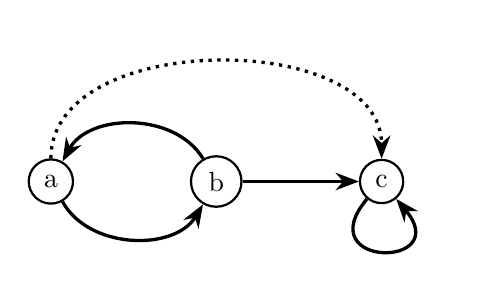
\begin{tikzpicture}[scale=0.70]
\begin{scope}[every node/.style={circle,thick,draw}]
    \node (A) at (0,0) {a};
    \node (B) at (3,0) {b};
    \node (C) at (6,0) {c};
\end{scope}

\begin{scope}[>={Stealth[black]},
              every node/.style={fill=white,circle},
              every edge/.style={draw=black,very thick}]
    \path [->] (A) edge[bend right=60] (B);
    \path [->] (B) edge[bend right=60] (A);
    \path [->] (B) edge[bend right=0] (C);
    \path [->] (A) edge[bend right=-90, dotted] (C);
    \path [->] (C) edge[loop below, in=-50,out=-130, looseness=8] (C);
\end{scope}
\end{tikzpicture}
\end{figure}

\end{frame}

\note[itemize]{
\item \Customorder{} can be defined as a total order on the partition of a set
\item This means that \customorder{} on the instantiated rules is isomorphic to the \enquote{total-order} on a partition of instantiated rules
\item By partition, we mean an unordered set. So there is no order between instantiated rules that belong to the same inner set
\item Also notice in this picture we have loops, these are elements that are in a cycle
}

\begin{frame}{Schedule For CAG (This Thesis)}{Schedule for circular attribute grammar}

\begin{definition}\label{def:cag-schedule-definition}
A \emph{schedule} for a circular attribute grammar is a \customorder{} ($\lesssim$) on the set of instantiated rules.
\end{definition}

\newlinevspace

Schedule is valid when ($a < b$ is $a \lesssim b \wedge b \not \lesssim a$):

% TODO
\[\begin{cases}
      \hat{r_i} < \hat{r_j},    & \text{whenever } \hat{v}_k \in \mathit{DO}(\hat{r_i}) \wedge \hat{v}_k \in \mathit{SUO}(\hat{r_j}) \\
      \hat{r_i} \lesssim \hat{r_j}, & \text{whenever } \hat{v}_k \in \mathit{DO}(\hat{r_i}) \wedge \hat{v}_k \in \mathit{MUO}(\hat{r_j})  
    \end{cases}\]
    
\end{frame}


\note[itemize]{
\item Schedule for circular attribute grammar is a \customorder{} on the instantiated rules
\item Schedule is valid when dependencies are respected, meaning that simple or non-monotone uses are not involved in a cycle
\item Also, note that less than symbol $<$ here does not mean total order, instead it means something is less-sim $\lesssim$ another but not the other way around
\item I also did not use the word: \enquote{strict}
}


% trivial schedule can go to where you talk about circular stuff
\begin{frame}{Trivial Schedule}{Observation}

Only when \alert{all uses are monotone}

$$ \Big\{ \{ \hat{r_0}, \dots, \hat{r_7} \} \Big \}$$

This happens when for all $\hat{r_1}, \hat{r_2} \in \hat{R}$, $\hat{r_1} \lesssim \hat{r_2} \wedge \hat{r_2} \lesssim \hat{r_1}$.

\end{frame}

\note[itemize]{
\item In circular and circular remote attribute grammars, we can have a trivial schedule
\item Trivial schedule is when we have all monotone functions
\item Basically all instantiated rules may belong to the same level
\item So we just evaluate all instantiated rules over and over again until a fixed point is reached
}

\begin{frame}{$l$-Ordered Circular Attribute Grammars}{Definition of $l$-ordered for CAG}

$l$-ordered Circular Attribute Grammars requires:
\begin{itemize}
    \item Summary graph to be \customorder{}
    \item Augmented dependency for each production is a \customorder{} such that:
    \begin{itemize}
        \item All dependencies involved in cycles must be monotone
        \item Restricted \customorder{} of the augmented dependency graph for a non-terminal must be the same as the \customorder{} for the summary graph for that non-terminal
    \end{itemize}
\end{itemize}


\end{frame}

\note[itemize]{
\item In $l$-ordered circular attribute grammar, we are required to have a summary graph that is a \customorder{}
\item For every augmented dependency graph we can form a \customorder{} and all dependencies in the cycle have to be monotone 
\item Also, if we restrict the \customorder{} of the augmented dependency graph to just one of the non-terminals, it should be the same \customorder{} for the summary graph
}

\begin{frame}[fragile=singleslide]{CAG Example}{CAG example with 2 independent cycles}



\begin{multicols}{2}
\begin{Verbatim}[fontsize=\small]
S -> A A
    A0.i1 = A1.s1
    A0.i2 = A1.s2
 
    A1.i1 = A0.s1
    A1.i2 = A0.s2

    S.s = A0.s1 + A0.s2

A -> a
    A.s1 = A.i1
    A.s2 = A.i2





\end{Verbatim}
\end{multicols}
    
\end{frame}

\note[itemize]{
\item As an exercise, let's analyze this circular attribute grammar
\item Notice that there are two independent cycles involving $i_1$, $s_1$ and another cycle involving $i_2$, $s_2$
\item To resolve $A_1.s_1$ we need to resolve $A_1.i_1$ and to resolve that we need to resolve $A_0.s_1$ and to resolve that we need to resolve $A_1.s_1$, hence the cycle as we write to $A_1.s_1$ using $A_1.s_1$.
\item There is a similar cycle involving attributes $i_2$ and $s_2$
}


\begin{frame}{CAG $l$-ordered}{ Summary graph for CAG example}
    Summary graph that is \customorder{} for non-terminal $A$



	\begin{figure}[htbp]
		\centering
		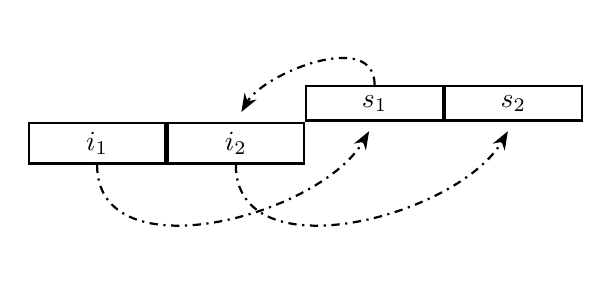
\begin{tikzpicture}[->,>=Stealth,auto,scale=0.6,shorten >= 4pt,
			thick,main node/.style={draw, rectangle, align=center}]

			\node[main node,text width=1.5cm] (1) at (0,0)    {$i_1$};
			\node[main node,text width=1.5cm, anchor=north west] (2) at(1.north east) {$i_2$};
			\node[main node,text width=1.5cm, anchor=south west] (3) at(2.north east) {$s_1$};
			\node[main node,text width=1.5cm, anchor=north west] (4) at(3.north east) {$s_2$};
		
			\draw[black, dash dot] (1.south) to[out=-90, in=-120,looseness=1] (3.south);
			\draw[black, dash dot] (2.south) to[out=-90, in=-120,looseness=1] (4.south);

   			\draw[black, dash dot] (3.north) to[out=90, in=60,looseness=1] (2.north);
		\end{tikzpicture} 
		
		\caption{$\mathit{SDG}_A$}
	\end{figure}

\end{frame}
\note[itemize]{
\item Let's propose a summary graph for non-terminal $A$ that captures all possible dependencies among its attribute 
}



\begin{frame}{CAG $l$-ordered}{ Augmented dependency graph for CAG example}

    $\mathit{ADG}_{S \to AA}$: Augmented dependency graph for $S \to A A$

	\begin{figure}[htbp]
		\centering
		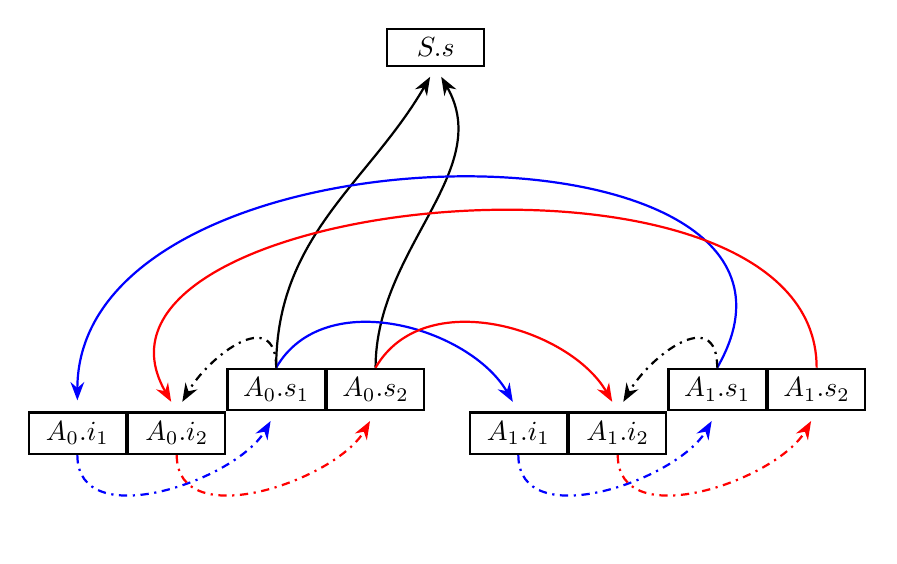
\begin{tikzpicture}[->,>=Stealth,auto,scale=0.35,shorten >= 4pt,
			thick,main node/.style={draw, rectangle, align=center}]
			
			\node[main node,text width=1cm] (1) at (5,14)    {$S.s$};
			
			
			\node[main node,text width=1cm] (2) at (-8,0)    {$A_0.i_1$};
			\node[main node,text width=1cm, anchor=north west] (3) at(2.north east) {$A_0.i_2$};
			\node[main node,text width=1cm, anchor=south west] (4) at(3.north east) {$A_0.s_1$};
			\node[main node,text width=1cm, anchor=north west] (5) at(4.north east) {$A_0.s_2$};
			
			\node[main node,text width=1cm] (6) at (8,0)    {$A_1.i_1$};
			\node[main node,text width=1cm, anchor=north west] (7) at(6.north east) {$A_1.i_2$};
			\node[main node,text width=1cm, anchor=south west] (8) at(7.north east) {$A_1.s_1$};
			\node[main node,text width=1cm, anchor=north west] (9) at(8.north east) {$A_1.s_2$};
			
			\draw[black] (4.north) to[out=90, in=-120,looseness=1] (1.south);
			\draw[black] (5.north) to[out=90, in=-60,looseness=1] (1.south);

			\draw[blue] (8.north) to[out=60, in=90,looseness=1.2] (2.north);
			\draw[red] (9.north) to[out=90, in=120,looseness=1] (3.north);

			\draw[blue] (4.north) to[out=60, in=120,looseness=1] (6.north);
			\draw[red] (5.north) to[out=60, in=120,looseness=1] (7.north);
   
			\draw[blue, dash dot] (2.south) to[out=-90, in=-120,looseness=1] (4.south);
			\draw[red, dash dot] (3) to[out=-90, in=-120,looseness=1] (5.south);

			\draw[blue, dash dot] (6.south) to[out=-90, in=-120,looseness=1] (8.south);
			\draw[red, dash dot] (7.south) to[out=-90, in=-120,looseness=1] (9.south);
   
			\draw[black, dash dot] (4.north) to[out=90, in=60,looseness=1.5] (3.north);
			\draw[black, dash dot] (8.north) to[out=90, in=60,looseness=1.5] (7.north);
   
		\end{tikzpicture} 
		
	\end{figure}
	

    
\end{frame}
\note[itemize]{
\item Notice this dependency graph is definitely a \customorder{}
\item There are two independent cycles: red and blue
\item These cycles became total thanks to the two edges (colored in black) from $A_0.s_1$ to $A_0.i_2$ and similarly $A_1.s_1$ to $A_1.i_2$, these two edges came from the summary dependency graph of non-terminal $A$
\item If we restrict the augmented dependency graph to just non-terminal $A$, we will get back the same \customorder{} that was given in the summary graph of $A$, hence this circular attribute grammar is $l$-ordered
}

\begin{frame}{\Customorder{} in $\mathit{ADG}$}

    \Customorder{} in the $\mathit{ADG}_{S \to AA}$
    
\[ \bigg \{  \big \{ A_0.i_1, A_0.s_1, A_1.i_1, A_1.s_1 \big \} < \big \{ A_0.i_2, A_0.s_2, A_1.i_2, A_1.s_2 \big \} < S.s \bigg \} \]


\end{frame}

\note[itemize]{
\item This is the \customorder{} of the augmented dependency graph we saw in the previous slide as a total order on the partition of the set
\item Notice that we have two independent cycles and they appear in-order 
}

\begin{frame}{$l$-Ordered Circular Attribute Grammars}{Extending definition of $l$-ordered to circular AGs (CAG)}
    
    \begin{lemma}\label{cag-lordered-wellformed}
$l$-ordered circular attribute grammars are well-formed.
\end{lemma}
\newlinevspace
    Constructive proof with contradictions in case analysis.
    
\end{frame}

\note[itemize]{
\item Lastly, we \textbf{proved} in the thesis that the definition of $l$-ordered can be extended to circular attribute grammars and its well-formed
}

\subsection*{Circular Remote AG}{}

\begin{frame}{Extensions Overview}{Classical AG extensions}
     \begin{description}
        \item $\checkmark$ Classical attribute grammar
        \item $\checkmark$  Remote attribute grammars
        \item $\checkmark$ Circular attribute grammars
        \item $\square$   \alert{Circular remote attribute grammars}
    \end{description}
\end{frame}

\note[itemize]{
\item Next, we are going to describe circular remote attribute grammars
}


\begin{frame}{Circular Remote Attribute Grammar}{Definition: Circular + Remote AG}

\begin{definition}
A circular remote attribute grammar is an \alert{extension of remote attribute grammars} and has the same form as remote attribute grammars, except \alert{certain attributes are circular} and \alert{uses of attribute occurrences in functions are declared monotone in some arguments}.
\end{definition}
\end{frame}

\note[itemize]{
\item This is the informal definition of circular remote attribute grammar or CRAG
\item It is a merge of two previous two extensions: circular and remote into one
\item This is the most accommodating extension to describe circularly defined problems over a tree
}

% TODO
\begin{frame}{Circular Remote Attribute Grammar}{Applications}
Applications for CRAG:

\begin{itemize}
    \item First and Follow sets
    \item Unification (in type inference)
	\item Sub-typing with circular types (a class extending its own generic parameter)
	\item Detecting circular class extension in COOL semantic analyzer (e.g. A extends B, B extends C, C extends A)
 \item Program control-flow analysis
\end{itemize}
\end{frame}

\note[itemize]{
\item There are many applications for a circular remote attribute grammar including First and Follow in parsing, unification in type inference, detecting circularly defined class hierarchy during type checking, and control flow analysis
% \item COOL is a programming language (classroom object-oriented language)
}


\begin{frame}[fragile=singleslide]{Circular Remote Attribute Grammar}{Evaluation strategy}
Hedin in \cite{10.1016/j.scico.2005.06.005} used fixed-point loops with \alert{demand evaluation} to evaluate circular remote attribute grammar.

\begin{Verbatim}[fontsize=\small]
    do {
    
        // Evaluate rules (again?)
        
    } while (currentValue \supset prevValue)
\end{Verbatim}

\newlinevspace

But, what about \alert{schedule}? how to formalize the validity of the schedule for CRAG?
\end{frame}

\note[itemize]{
\item In CRAG, similar to circular attribute grammars, we need a fixed point loop for evaluation
\item This is the basic setup of a fixed-point loop introduced by Hedin
\item Basically, we hold on to the previous value and then run the evaluation and then check whether the new value is a superset, NOT superset-equal to the previous value. And if that is the case then we re-run the loop.
}



\begin{frame}{Circular Remote Attribute Grammar}{Evaluation Terminating? Monotonicity}

\begin{block}{Remark}
The partial field write rule as defined in the definition of remote attribute grammar is a \alert{monotone} use.
\end{block}

\end{frame}

\note[itemize]{
\item Adding a monotonicity constraint ensures that fixed-point evaluation terminates
\item However, partial field writes are monotone, this is because object fields are \enquote{set} so they can be involved in a cycle
\item The only thing remaining is ensuring that arguments of semantic functions are monotone in a classical rule
}






\begin{frame}{Circular Remote Attribute Grammar}{Schedule Definition}
    
\begin{definition}
A schedule for a circular remote attribute grammar is a \alert{\customorder{}} $\lesssim$ on the \alert{instantiated rules}.
\end{definition}


Schedule is valid when ($a < b$ is $a \lesssim b \wedge b \not \lesssim a$):

% TODO: the same as 38
\[\begin{cases}
      \hat{r_i} < \hat{r_j},    & \text{whenever we have a simple dependency} \\
      \hat{r_i} \lesssim \hat{r_j}, & \text{whenever we have a monotone dependency}
    \end{cases}\]

    And for any two rules $\hat{r}_i = (v \texttt{=} w.f)$, $\hat{r}_j = (w'.f \sqsupseteq v' ) \in R(t)$ if these rules are \alert{potentially} referring to the same object then $\hat{r}_j \lesssim \hat{r}_i$ 

\end{frame}

\note[itemize]{
\item Schedule for CRAG is a \customorder{} of instantiated rules
\item Schedule is valid when dependencies defined using $\mathit{DO}$ and $\mathit{UO}$ are respected meaning that the definition of attribute instance precedes the use of the same attribute instance
\item And similarly writes to field of an object should precede the read of the field of the same object
}



% keep this :)
\begin{frame}[fragile=singleslide]{Example}{CRAG Example}

\begin{multicols}{3}
\begin{Verbatim}[fontsize=\small]
S -> A B
    local l
    l = A.r
    B.i = l
    A.i = B.s
    S.x = l.f
A -> a
    object o
    o.f <- A.i
    A.r = o


B -> b
    local l
    l = B.i
    B.s = l.f
\end{Verbatim}
\end{multicols}

\newlinevspace

$\Rightarrow$ Notice the \alert{cycle} involving reading and writing of the same object

\end{frame}

\note[itemize]{
\item This is an example of circular remote attribute grammar
\item Notice $o.f$ gets $A.i$ using partial field write and $A.i$ itself gets $B.s$ using classical rule
\item Then $B.s$ gets $l.f$ where $l$ is a local attribute assigned
\item Basically, we write to $o.f$ using the value of $o.f$. Hence a cycle.
}


% kill this
\begin{frame}[fragile=singleslide]{Example}{Instantiated CRAG with trivial derivation}

\begin{multicols}{3}
\begin{Verbatim}[fontsize=\small]
n0: S -> A B
    local l0
    r0: l0 = n1.r
    r1: n2.i = l0
    r2: n1.i = n2.s
    r3: n0.x = l0.f
n1: A -> a
    object o0
    r4: o0.f <- n1.i
    r5: n1.r = o0


n2: B -> b
    local l1
    r6: l1 = n2.i
    r7: n2.s = l1.f
\end{Verbatim}
\end{multicols}

Schedule: 

\[
     \Big \{ \{ \hat{r}_5 \} < \{ \hat{r}_0 \} < \{ \hat{r}_1 \} < \{ \hat{r}_6 \} < \{ \hat{r}_4 , \hat{r}_7, \hat{r}_2 \} < \{ \hat{r}_3 \}  \Big \}
\]

\end{frame}

\note[itemize]{
\item This is the instantiated form of the circular remote attribute grammar we introduced in the previous slide
\item The corresponding schedule is at the bottom
\item Remember that \customorder{} is a total-order on a partition, hence why we used less-than $<$ here
}




% kill this
\begin{frame}[fragile=singleslide]{Example}{CRAG Example with non-monotone function $h$}

\begin{multicols}{3}
\begin{Verbatim}[fontsize=\small]
n0: S -> A B
    local l
    r0: l = h(n1.r)
    r1: n2.i = h(l)
    r2: n1.i = n2.s
    r3: n0.x = h(l.f)
n1: A -> a
    object o
    r4: o.f <- n1.i
    r5: n1.r = h(o0)


n2: B -> b
    local l
    r6: l = h(n2.i)
    r7: n2.s = l.f
\end{Verbatim}
\end{multicols}

\newlinevspace

The \textbf{trivial schedule} \alert{does not work} for this example because of $h$

\end{frame}

\note[itemize]{
\item If we introduce non-monotone function $h$ in a cycle, this means that the trivial schedule is no longer applicable or valid
}


\begin{frame}{$l$-Ordered Circular Remote Attribute Grammars}{Extending definition of $l$-ordered to circular remote AGs (CRAG)}
    
    \begin{lemma}\label{crag-lordered-wellformed}
$l$-ordered circular remote attribute grammars are well-formed.
\end{lemma}
\newlinevspace
    Proof by applying \enquote{fiber construction} and \enquote{fiber approximation} to proof of $l$-ordered circular attribute grammars
    
\end{frame}

\note[itemize]{
\item Lastly, we showed in the thesis that definition of $l$-ordered can be extended to circular remote attribute grammars thanks to \enquote{fiber-construction} and \enquote{fiber-approximation}
}

\section{Methods}



\subsection*{Fibers}{}

\begin{frame}{Methods Overview}{Methods and algorithms}
     \begin{description}
        \item $\square$ \alert{Fiber cycle breaking}
        \item $\square$  Visit sequences
        \item $\square$  SCC chunk scheduling
    \end{description}
\end{frame}

\note[itemize]{
\item Next, we are going to talk about fiber cycles 
}

\begin{frame}{Fiber Construction}{Informal Definition: Beyond the scope of this presentation}

\small
\begin{itemize}
    \item A construction that expresses the semantics of \emph{remote attribute grammars} in \emph{classical terms}
    \item Objects \alert{implicitly} carry separate values for the fields is like a \alert{rope} which can be separated into the individual fibers
    \item This yields an improper attribute grammar with an infinite number of attributes
    \item \emph{fiber approximation} fixes that (which then may include \alert{fiber cycles})
\end{itemize}

\begin{center}
\includegraphics[scale=0.2]{rope-fiber.png}
\end{center}
    
\end{frame}

\note[itemize]{
    \item I am intentionally not going into details of fiber-construction because it would be a disservice to remote attribute grammar paper
    \item Basically, it expresses the semantics of remote attribute grammars in classical terms
    \item It is called \enquote{fibers} because objects implicitly carry separate values for the fields and it is like a rope that can be separated into individual fibers
    \item But fiber-construction yields an improper attribute grammar with an infinite number of attributes
    \item Then fiber-approximation fixes that but it then may include \alert{fiber-cycles}
}


% 

\begin{frame}{Fiber Cycle Breaking}{Benign fiber cycles are okay for scheduling}

\alert{Fiber attributes} guide the scheduler and have no run-time significance

\newlinevspace

\begin{itemize}
    \item % some cycles are benine because they only consist of fiber attruibyres
Before in RAG, some cycles can be ignored because they entirely involve so-called fiber attributes

\newlinevspace

%  in existing APS systsme, they can be scheduled using a hack that added new attributes UP and DOWN to break cycles
%  in this work we found we didn't need this hack, we found that we can handle them generalkly because they are monotone
% fiber attributes
    \item In CAG (or CRAG), some cycles may \alert{carry value} and this will have run-time significance
\end{itemize}
\end{frame}

\note[itemize]{
\item Even in a remote attribute grammar that is non-circular we may have pure fiber cycles and it's okay.
\item Fiber cycles are different between remote attribute grammar and circular remote attribute grammar because in the latter case, they may carry value
}



\begin{frame}{Fiber Cycle Breaking}{Issue with existing static scheduler}

Previously in RAG:
\begin{itemize}
    \item For every non-terminal whose fibered attributes take part in the cycle, created two \alert{AST nodes} called up and down and connected all nodes to these to break cycles and \alert{preserve only UP followed by DOWN}.
\end{itemize}


\end{frame}

\note[itemize]{
\item Previously for remote attribute grammars, fiber cycles were broken and to do that two artificial attributes called UP and DOWN would be created. This introduced a lot of implementation complexity
\item To fix that we wrote a new algorithm that treats all attributes as either UP or DOWN and it simplifies fiber cycle breaking
}



% kill this
% \begin{frame}{Fiber Cycle Breaking}{Validated with RAG!}

% \alert{Drop-in replacement} algorithm was successful in APS.

% \begin{itemize}
%     \item Validated the algorithm against \alert{previous APS codes} that contained only fiber cycles
% \end{itemize}

% \end{frame}

% \note[itemize]{
% \item We tested the fiber cycle breaking algorithm against APS examples that contained only fiber cycles
% \item And it was successful 
% }



\begin{frame}{Fiber Cycles Are Monotone}{CRAG static scheduler can handle fiber cycles}
    \textbf{But} this turned out to be \alert{unnecessary} because fiber dependencies are \alert{monotone} and can be handled by the new CRAG scheduler, so this change was not necessary. 

\newlinevspace
Welcome outcome.
    
\end{frame}

\note[itemize]{
\item But the whole fiber cycle breaking change turned out to be unnecessary and not needed because fiber cycles are monotone and can be handled by the CRAG static scheduler
\item This is welcome news because the simpler the implementation, the better
}
\subsection*{Visit Sequences}{}

\begin{frame}{Methods Overview}{Methods and algorithms}
     \begin{description}
        \item $\checkmark$ Fiber cycle breaking
        \item $\square$  \alert{Visit sequences}
        \item $\square$  SCC chunk scheduling
    \end{description}
\end{frame}

\note[itemize]{
\item Next, we are going to talk about visit sequences
}

\begin{frame}{Visit Sequence Evaluation}{Static evaluator based on $l$-ordered evaluation class}

$\Rightarrow$ \alert{Visit sequence evaluation} is a type of \alert{static evaluation}

\newlinevspace

Pros:
\begin{itemize}
    \item Evaluation \alert{will terminate}
    \item \alert{No re-evaluation}
    \item Better space complexity as runtime dependencies are not stored
    \item Time complexity of: $\mathcal{O}(| \hat{R} |)$ (for classical AG)
    \item \alert{Practical}: can be generated independent of derivation
\end{itemize}

Cons:
\begin{itemize}
    \item Requires extensive static analysis of attribute grammars
\end{itemize}
\end{frame}

\note[itemize]{
\item Kastens introduced $l$-ordered class of attribute grammars and introduced a type of static evaluator called a visit sequence evaluator
\item Visit sequence evaluator does not need a runtime dependency analysis so it has a better space and time complexity compared to demand evaluation
\item And runs in linear time for a classical attribute grammar
\item And can be generated once and works for all derivations of a grammar
\item But only works for $l$-ordered evaluation class of attribute grammars
}


% visit sequence is a series of recursive function where each each non-terminal is visited fixed number of times and each visit can visit the children, and in the end all visits are done for every node of the tree
\begin{frame}[fragile=singleslide]{Example}{Visit sequence evaluator}

Set of \alert{recursive functions} where each function takes an \alert{instance of non-terminal} (derivation tree node)

{\tiny
\begin{multicols}{2}
\begin{Verbatim}[fontsize=\scriptsize]
visit_S(n: S -> A)
    A.i1 = S.in
    visit_A_part1(A)
    A.i2 = A.s1
    visit_A_part2(A)
    S.out = A.s2

visit_A_part1(n: A -> A A)
    A1.i1 = A0.i1
    visit_A_part1(A1)
    A1.i2 = A1.s1
    visit_A_part2(A1)
    A0.s1 = A1.s2
visit_A_part2(n: A -> A A)
    A2.i1 = A0.i2
    visit_A_part1(A2)
    A2.i2 = A2.s1
    visit_A_part2(A2)
    A0.s2 = A2.s2

visit_A_part1(n: A -> 'a')
    A.s1 = A.i1 + 1

visit_A_part2(n: A -> 'a')
    A.s2 = A.i2 + 1
    
\end{Verbatim}
\end{multicols}
}

\end{frame}

\note[itemize]{
\item This is a visit sequence evaluator for the classical attribute grammar we described previously
\item Notice that we have 4 recursive functions, each function takes an attribute instance associated with a production and then evaluates some of its attributes inside the visit function
\item We have 5 recursive functions in this example
\item We also see that visit $A$ has part $1$ and part $2$ and that corresponds to phase $1$ and phase $2$ of the summary graph schedule
}


\begin{frame}{Visit Sequence}{Protocol is like an interface}

\begin{definition}
A \emph{Protocol} $\Pi(X)$ is an \alert{ordered partition of attributes} for each non-terminal $X \in N$, where it can include an empty set or multiple synthesized or inherited attributes.
\end{definition}

$\rightarrow$ inherited and synthesized are packaged together
\begin{itemize}
    \item \alert{inherited goes in} and \alert{synthesized goes out}
\end{itemize}


For example, $\Pi(A)$ is the following:
\[ \Pi(A) = \Big\{ \{ A.i_1, A.s_1 \} < \{ A.i_2, A.s_2 \} \Big\} \]

Visit Sequence has to be compatible with $\mathit{Ord}(R(p))$ and $\Pi(X_i)$

\end{frame}

\note[itemize]{
\item To understand a visit sequence we first need to understand a protocol which is like an interface in a programming language
\item A protocol for a non-terminal is an ordered partition of attributes, this may include an empty set or set containing multiple synthesized or inherited attributes
\item Protocol for a non-terminal is just like a package of inherited and synthesized attributes. Inherited goes in and synthesized comes out
\item A visit sequence for a production has to be compatible with an ordered set of all rules associated with a production $R(p)$ and protocol for all non-terminals involved in a production
\item We call each inner-set in the protocol a \textit{phase}
}


\begin{frame}{Visits for Classical AG}{Definition of visit sequence for classical AG}

A \emph{visit-sequence} $\mathscr{V}(p)$ for $p{:} X \rightarrow \alpha \in P$ of a $l$-ordered AG is:

\begin{itemize}
    \item a sequence of visits where each visit consists of
    \begin{itemize}
        \item rules that define local attributes
        \item rules that define/use child inherited/synthesized attributes 
        \item child visit call of a particular phase
    \end{itemize}
\end{itemize}


{
\scriptsize
\begin{equation}\label{eq:visit-for-production-aa}
\begin{gathered}
\mathscr{V}(p{:} A_0 \rightarrow A_1 A_2) = \Bigg\{               
   \overbrace{ \Big\{  \mathit{visit}(A_1, 1)  < \mathit{visit}(A_1, 2)	 \Big\}}^\text{first visit corresponding to first set in $\Pi(A)$ }  <  \\
   \underbrace{ \Big\{  \mathit{visit}(A_2, 1)  < \mathit{visit}(A_2, 2) \Big\}}_\text{second visit corresponding to second set in $\Pi(A)$}
\Bigg\}
\end{gathered}
\end{equation}
}

\begin{itemize}
    \item[] {\huge \bell}  $\mathit{visit}(A_1, 2)$: visit function for phase 2 of $A$ taking an instance of non-terminal $A$ with production index $1$
\end{itemize}
\end{frame}

\note[itemize]{
\item Visit sequence is a sequence of visits
\item Each visit may contain rules or child visit call for a particular phase
% \item By rules we mean rule that define local attributes, or rules that define child inherited attributes or rules that use child synthesized attributes or rules that define parent synthesized attributes, so all of that
\item In this example, we have a visit sequence with two visits, because the protocol for the LHS non-terminal of the production had two phases
\item Each visit is corresponding to a phase or set in the protocol
\item For example, visit one is corresponding to phase one of the protocol
}


\begin{frame}{Protocol for CRAG}{CRAG protocols can have empty phases}

\begin{definition}
\emph{Protocol} $\Pi(X)$ for each non-terminal $X \in N$ of circular remote attribute grammar is a \alert{sequence of possibly empty sets} of attributes of non-terminal where some of the sets are marked as cyclic.
\end{definition}

Empty phase in protocol:
\begin{itemize}
    \item start and end with non-circular phase
    \item empty phase between two circular phases to make sure cycles do not get merged
\end{itemize}

\end{frame}


\note[itemize]{
\item Protocol for CRAG is different from protocol in classical AG because it has to accommodate cycles
\item To that we mark each inner-set in the protocol as circular or non-circular
\item And then we need to make sure the protocol start and end with non-circular phase, if there is none then we can just stick an empty non-circular phase at the start or end
\item Similarly, to make sure separate cycles do not get merged, so we add an empty non-circular phase between two circular phases
\item To allow one time semantic rule like local attribute otherwise there is no place to put it
}



\begin{frame}{Example of Protocol for CRAG}

\begin{equation}\label{eq:protocol-for-crag-example}
\begin{gathered}
\Pi(S) =  \Big \{   \overbrace{\{ S.x \} }^{\text{non-circular visit}}     \Big \} \\
\Pi(A) =  \Big \{  
\overbrace{\big \{  A.r  \big \}}^{\text{empty non-circular visit}} <
\overbrace{\big \{  \underbrace{  \{  A.i  \}}_{\text{cycle}}  \big \}}^{\text{circular visit}} <
\overbrace{\big \{    \big \}}^{\text{empty non-circular visit}}
\Big \} \\
\Pi(B) =  \Big \{
\overbrace{\big \{   B.i  \big \}}^{\text{empty non-circular visit}} <
\overbrace{\big \{  \underbrace{  \{  B.s \}}_{\text{cycle}}  \big \}}^{\text{circular visit}} <
\overbrace{\big \{    \big \}}^{\text{empty non-circular visit}}
\Big \} \\
\end{gathered}
\end{equation}
    
\end{frame}

\note[itemize]{
\item This is a protocol for each non-terminal of circular remote attribute grammar we previously saw
\item Notice that each set is marked as circular or non-circular and we start and end with non-circular phase
}

\begin{frame}{Visits for CRAG}{Definition of visit sequence for CRAG}

A \emph{visit-sequence} $\mathscr{V}(p)$ for $p{:} X \rightarrow \alpha \in P$ of $l$-ordered circular remote attribute grammar is:

\begin{itemize}
    \item an ordered set of visits similar to visit sequence for classical AG but:
    \begin{itemize}
        \item inside in each visit there can additionally be a sub-sequence of rules or child visits
        \item Inside this sub-sequence, there cannot be another level sub-sequence \item Each visit of each child occurs exactly once and they appear in the exact order they appear in the protocol.
    \end{itemize}
\end{itemize}

\end{frame}

\note[itemize]{
\item Visit sequence for circular remote attribute grammar is different from visit sequence for classical attribute grammar in  sense that it can include sub-sequences
\item Sub-sequences cannot include another level of sub-sequence
}


\begin{frame}{Visits for CRAG}{Visits in CRAG may contain sub-sequence}


{
\scriptsize
\begin{equation}\label{eq:visit-sequence-for-crag-example}
\begin{gathered}
\mathscr{V}(p{:} S \rightarrow A B) = \Biggl\{
\overbrace{
\begin{aligned}
\Bigl\{
 \mathit{visit}(A, 1)  < (l \texttt{=} A.r) < (B.i \texttt{=} l) < \mathit{visit}(B, 1) < \\
\underbrace{\{ \mathit{visit}(A, 2)   , \mathit{visit}(B, 2), (A.i \texttt{=} B.s)  \}}_{\text{sub-sequence cycle (fixed-point loop needed)}}   < \\
\mathit{visit}(A, 3)  < \mathit{visit}(B, 3) < \\
(S.x \texttt{=} l.f)
\Bigr\}
\end{aligned}
}^{\text{single parent visit corresponding to $\Pi(S)[0]$}}
\Biggr \} \\
\mathscr{V}(p{:} A \rightarrow a) = \Biggl\{
\overbrace{\Big \{  (A.r \texttt{=} o)  \Big \}}^{\text{non-circular visit}} <
\overbrace{\Big \{  (o.f \sqsupseteq A.i)   \Big \} }^{\text{visit}} <
\overbrace{\Big \{    \Big \}}^{\text{empty non-circular visit}}
\Biggr\} \\
\mathscr{V}(p{:} B \rightarrow b) = \Biggl\{
\overbrace{\Big \{  
(l \texttt{=} B.i )
\Big \}}^{\text{non-circular visit}} <
\overbrace{\Big \{  (B.s \texttt{=} l.f)  \Big \} }^{\text{visit}} <
\overbrace{\Big \{    \Big \}}^{\text{non-circular visit}}
\Biggr\}
\end{gathered}
\end{equation}
}
 
\end{frame}


\note[itemize]{
\item This is the visit sequence for the circular remote attribute grammar we previously saw
\item Notice we have some empty visits corresponding to empty phases in the protocol
\item Also each visit in the visit sequence corresponds to the protocol of the LHS non-terminal of the production
\item Lastly we have a sub-sequence in the first visit sequence 
}


\begin{frame}[fragile=singleslide]{Visit Sequence}{Visit sequence for circular remote AG}

{\scriptsize
\begin{figure}[htbp]
    \centering
\begin{multicols}{2}
\begin{verbatim}
visit_S(n: S -> A B)
    visit_A_1(A)
    l = A.r
    B.i = l
    visit_B_1(B)

    cycle:
        visit_A_2(A)
        visit_B_2(B)
        A.i = B.s

    visit_A_3(A)
    visit_B_3(B)
    S.x = l.f



visit_A_1(n: A -> a)
    o = new O()
    A.r = o

visit_B_1(n: B -> b)
    l = B.i

visit_A_2(n: A -> a)
    o.f <- A.i

visit_B_2(n: B -> b)
    B.s = l.f

visit_A_3(n: A -> a)

visit_B_3(n: B -> b)

\end{verbatim}
\end{multicols}
\end{figure}
}

\end{frame}

\note[itemize]{
\item This is the same visit sequence as a code, notice that we mark the sub-sequence as a cycle
}
\subsection*{SCC-Chunk Scheduling}{}

\begin{frame}{Methods Overview}{Methods and algorithms}
     \begin{description}
        \item $\checkmark$ Fiber cycle breaking
        \item $\checkmark$  Visit sequences
        \item $\square$  \alert{SCC chunk scheduling}
    \end{description}
\end{frame}

\note[itemize]{
\item Next, we are going to discuss SCC chunk scheduling and how it's working
}


\begin{frame}{Group Scheduling}{Simpler way to static schedule}

In each visit of the visit sequence:
\begin{itemize}
    \item whole group of parent inherited
    \item whole group of parent synthesized
    \item locals (i.e. local attributes and conditionals)
    \item child inherited and synthesized
\end{itemize}
\end{frame}

\note[itemize]{
\item Let's talk about group scheduling, instead of greedy scheduling individual attributes, we can schedule them as a group
\item In each visit of visit sequence there are 4 possible groups: parent inherited, parent synthesized, locals, and child visits (i.e. package of child inherited and synthesized attributes)
\item Attribute is ready to be scheduled when its dependencies are scheduled
\item So instead of checking if an attribute is ready, we say a group of attributes is ready to be scheduled when they are all ready 
\item This greatly simplifies the static schedule generation
}


\begin{frame}{SCC Chunk Scheduling Goal}{What is the end goal?}
    \begin{itemize}
        \item We want to follow group scheduling
        \item We want to preserve scoping for locals (e.g. IF statement)
        \item Circular attributes that are in a cycle with each other need to be scheduled together
    \end{itemize}
\end{frame}

\note[itemize]{
\item An ideal static scheduling algorithm:
\begin{itemize}
    \item Should follow group scheduling
    \item Should preserve locals for scoping purposes
    \item And circular attributes that are involved in a cycle should be scheduled together
\end{itemize}
\item And that is the goal of the SCC chunk scheduling algorithm that we designed
}


\begin{frame}{Chunks}{Chunks as a way of scheduling groups}
    What are the chunks?
    \newlinevspace{}

    \begin{itemize}
        \item \alert{Half-left}: parent inherited attributes for a particular phase
        \item \alert{Half-right}: parent synthesized attributes for a particular phase
        \item \alert{Child visit}: contain child inherited and synthesized for a given phase of a particular child
        \item \alert{Local}: contain a single local attribute
    \end{itemize}
\end{frame}

\note[itemize]{
\item We introduce the concept of chunks
\item There are four types of chunks. Half-left, half-right, visit chunks and locals
}


\begin{frame}{Chunk Graph}{Reflect attribute dependencies into chunk graph}

\begin{figure}
    \centering
\begin{tikzpicture}[%
node distance = 10mm and 12mm,
  start chain = A going below,
   arr/.style = {-Stealth, shorten >=1mm, shorten <=1mm},
   box/.style = {draw, semithick, align=center,
                 minimum height=6mm, text width=23em},
     C/.style = {circle, draw=black!50, semithick, node contents={}},
every join/.style = {arr}
                        ]
    \begin{scope}[nodes={on chain=A}]
\coordinate (aux);
\node[box]  {Create Chunks};   % A-2
\node[box, join]  {Bring Attribute Dependencies to Chunks};
\node[box, join]  {Add Guiding Dependencies to Chunks}; % A-4
\node[box, join]  {Find Strongly Connected Regions in Chunk Graph}; % A-4
    \end{scope}
\end{tikzpicture}
\end{figure}


\end{frame}

\note[itemize]{
\item The first step in our static scheduling algorithm is to create chunks
\item If LHS non-terminal has $n$ phases or inner-sets in its protocol, then we create $n$ half-left and $n$ half-right corresponding to each phase
\item For each non-terminal appearing on the RHS, we construct visit chunks where each visit chunk has a corresponding child index and phase number
\item Each local attribute belongs to its own chunk
\item Then we reflect attribute dependencies into the chunk graph, basically, if two attributes have a dependency then their belonging chunks have to include that dependency
\item Next we add guiding dependencies because remember some chunks may be empty because we may have added some empty phases in their corresponding protocol
\item These guiding dependencies ensure that visits appear consecutively even though some may be empty
\item Next we find strongly connected components of the chunk graph
}

\begin{frame}{Scheduling Circular vs. Non-Circular Phase}
    \begin{itemize}
        \item \alert{Circular phase}
            \begin{itemize}
                \item One large SCC component containing half-left, half-right, visits and locals and then group scheduling attributes in this SCC
            \end{itemize}
        \item \alert{Non-circular phase}
        \begin{itemize}
            \item Greedy group scheduling attributes 
        \end{itemize}
    \end{itemize}
\end{frame}

\note[itemize]{
 \item We have to distinguish between circular and non-circular parent phases
 \item If the parent phase or protocol inner-set at a particular index is circular, then we should have a single strongly connected component containing both half-left and half-right for this phase and (in-between) its child visits
 \item If the parent phase is non-circular then we should greedy schedule attributes
 }

\begin{frame}[fragile=singleslide]{SCC Chunk Scheduling high-level}{Algorithm that makes scheduling CRAG possible}

    \begin{tikzpicture}[%
node distance = 8mm and 12mm,
  start chain = A going below,
   arr/.style = {-Stealth, shorten >=1mm, shorten <=1mm},
   box/.style = {draw, semithick, align=center,
                 minimum height=6mm, text width=9em},
     C/.style = {circle, draw=black!50, semithick, node contents={}},
every join/.style = {arr}
                        ]
    \begin{scope}[nodes={on chain=A}]
\coordinate (aux);
\node[box]  {SCC Scheduling};   % A-2
\node[box, join]  {Chunk Scheduling};
\node[box, join]  {Group Scheduling}; % A-4
    \end{scope}
\node (in)  [C, left =of A-2, 
             label=left: Start];
\node (out) [C, right=of A-4,
             label=right:End];
%%%%
\draw[arr]  (in)  -- (A-2);
\draw[arr]  (A-4) -- (out);

\draw[arr]  (A-3.east) -|-[distance=-6em] (aux) 
                node[pos=0.5, right, align=left] {Loop SCC\\ for each Chunk}
                        -| ($(in)!0.5!(A-2.west)$); 
\draw[arr]  (A-4.west) -|-[distance=-6em] ($(A-2.south)!0.5!(A-3.north)$)
                node[pos=0.5, left, align=right] {Loop Chunk\\ for each Group};

\end{tikzpicture}
\end{frame}

\note[itemize]{
 \item This is the high-level structure of the algorithm
 \item Notice that we first find the next ready-to-schedule chunk-component, then we find the next ready-to-schedule chunk, then we apply group scheduling, and then start all over, so it's a 3-step process
 \item The full algorithm is written in the methods chapter
 }



\begin{frame}{Fixed-Point Loops}{Case-by-case analysis of when the fixed-point loop is needed or not allowed}

{ \small
\begin{tabular}{|p{0.46\linewidth} | p{0.45\linewidth}|}
\hline
% https://tex.stackexchange.com/questions/33486
\multicolumn{1}{|c|}{Visit Type} & \multicolumn{1}{c|}{Fixed-Point Loop?}   \\ 
\hline\hline
Circular visit inside of circular visit & No fixed-point loop. Since the parent visit repeats the evaluation, its loop includes the child visit as well.\\ \hline
Non-circular visit in a circular visit & Not allowed. \\ \hline
Non-circular visit in a non-circular visit & No fixed-point loop. The visit has to be evaluated only once. \\ \hline
A circular visit in a non-circular visit & Needs a fixed-point loop. \\ \hline
\end{tabular} }

\end{frame}

\note[itemize]{
\item Interesting slide, hang around here
\item This table describes the case-by-case analysis of when the fixed-point loop is needed during the visit sequence evaluation
\item Notice that if a visit is circular and it is called from another circular visit then the fixed-point loop in the outer visit includes the child visit as well. And therefore no additional fixed-point loop in the child visit is required
\item Additionally, a non-circular visit is not allowed in a circular visit
\item Similarly, a circular visit in a non-circular visit requires a fixed-point loop
}
\section{Implementation}


\begin{frame}{Static Scheduler}{Simplify scheduling by using groups}

Previously:
\begin{itemize}
    \item Old greedy scheduler was \alert{tightly coupled with code generation} module
\end{itemize}
    
Now:
\begin{itemize}
    \item Scheduling is still greedy but it is using groups and is simpler, easier to debug, and \alert{de-coupled from code generation} module
    % \item Includes $(\mathit{ph}, \mathit{ch})$ marker to help code generation identify where a \alert{child visit} is happening and mark the \alert{end of parent visit}
\end{itemize}

\end{frame}


\note[itemize]{
\item Lets talk about the implementation of SCC chunk static scheduling in APS
\item The static scheduler or the module that constructs the visit sequences was tightly coupled with the code generation module and it was not working well
\item So we designed a replacement that is still greedy but simpler as it schedules instances as groups and uses visit markers to indicate where child visit happens and when parent visit ends
}




\begin{frame}{Static Schedule Assertions}{Ensuring greedy algorithm generates valid schedule}
    Due to the \alert{greedy nature of the static scheduler}, we included a series of \alert{assertions} to \alert{statically} (NOT during runtime) ensure the generated static schedule makes sense.

\newlinevspace
    
    \begin{itemize}
        \item No non-circular attribute in a circular parent visit
        \item Non-circular declared attributes may not participate in cycles
        \item Parent visits have to appear sequentially
        \item Child visits have to be invoked sequentially
        \item No missing parent and child visit
    \end{itemize}
\end{frame}

\note[itemize]{
\item Due to the greedy nature of our static scheduling algorithm we need some validation or assertions to make sure the generated schedule makes sense  
\item These validations are described in the thesis in the methods chapter
\item But some of these validations are described in this slide
}


\begin{frame}{\texttt{C} Code Statistic}{Basic Statistics About the New Scheduler}
    \begin{itemize}
        \item Old Scheduler only: $\approx500$ lines of \texttt{C} code
        \item New Static Scheduler + \alert{Assertions}: $\approx 3000$ lines of \texttt{C} code
    \end{itemize}
\end{frame}


\note[itemize]{
\item Here we have basic statistics about the new static scheduler algorithm implementation
\item Note that the number on the second line also includes various assertion functions as well
}

\begin{frame}[fragile=singleslide]{CRAG Scala Generated Evaluator}{Attribute Instance Setter + Monotonicity check}
\begin{Verbatim}[fontsize=\scriptsize]
// Template code to support static circular evaluation
// by building upon circular evaluation structure
var changed: Boolean = false;
trait StaticCircularEvaluation[V_P, V_T] extends CircularEvaluation[V_P, V_T] {
  override def set(newValue : ValueType): Unit = {
    val prevValue = value;
    super.set(newValue);
    changed |= prevValue != value;
  }

  override def check(newValue : ValueType): Unit = {
    if (value != null) {
      if (!lattice.v_equal(value, newValue)) {
        if (!lattice.v_compare(value, newValue)) {
          throw new Evaluation.CyclicAttributeException("non-monotonic " + name);
        }
      }
    }
  }
  
  // Do not treat multiple assignments of attributes as errors
  checkForLateUpdate = false;
}
\end{Verbatim}
\end{frame}


\note[itemize]{
\item (Skip this)
\item This is an example of an attribute instance setter, notice that we have a monotonicity checker that compares the old value with the new value to make sure the monotonicity requirement is being followed
\item Here we allow multiple attribute value assignments as this is an attribute that was declared circular 
\item We also have a global changed variable that we set if there was a \enquote{change} in attribute value after the assignment
\item In the next slide we will see how this \enquote{changed} global variable is being used
}

% kill scala codes, especially this
\begin{frame}[fragile=singleslide]{CRAG Scala Generated Evaluator}{Fixed-Point Loop around visits}
\begin{Verbatim}[fontsize=\scriptsize]
// Example of how child visits can be wrapped inside of the do-while loop
// Backup previous (global) changed value and run the code block at least once
val prevChanged_2_0 = changed;
do {
  changed = false;
  visit_4_2(v_prods);
} while (changed);
// Restore the changed value to ensure the fixed-point loop does not interfere
// with potential other fixed-point loops somewhere higher in the tree
changed = prevChanged_2_0;
\end{Verbatim}
\end{frame}

\note[itemize]{
\item (Skip this)
\item Notice that \enquote{changed} global variable is being backed up before we get to the fixed-point loop, and restored after the fixed-point loop
\item And then we see a do-while loop while there is a change somewhere in the attribute instances that are being re-evaluated during the visit subroutine call
}

\begin{frame}{Concession}{Concession in the implementation}
    \alert{Concession} in the implementation was \alert{no support for conditional cycles}

    \newlinevspace 
    Two situations can arise when using conditions with circular attribute grammars:
    
    \begin{itemize}
        \item[] \cmark \; \alert{Conditions inside the cycle}, which showcases the need to use direct edges for scheduling chunks because of potential scoping issues (\texttt{cycle-series.aps})
        \item[] \xmark \; Conditional cycles where the \alert{condition sits outside controlling the cycles}, this is where our APS implementation is not supported (\texttt{tiny-coag.aps})
    \end{itemize}
\end{frame}

\note[itemize]{
\item There are two possible types of conditions with cycles, we can have a condition inside the cycle and condition outside of the cycle. The first one is supported and the second on is not
\item This is a small concession in the implementation that we left-out as a future work
\item There is a graph of an example of such attribute grammar in the thesis
\item In APS, we statically detect if a given attribute grammar has this type of a condition and we throw an error
}

\section{Benchmarks}


\begin{frame}{Benchmark Workstation}{Desktop PC}


\begin{itemize}
    \item \texttt{i5-8500} CPU
    \item \texttt{32GB} of RAM
    \item \texttt{Ubuntu 22.04-LTS}
    \item \texttt{Scala 2.13.10} 
    \item \alert{JVM flags \texttt{-Xmx16g}}
    \item  No optional optimization flags
\end{itemize}
\end{frame}

\note[itemize]{
\item Next, let's talk about benchmarking our implementation
\item We used a Ubuntu workstation with \texttt{i5} CPU and 32 GB of RAM
\item The highlighted bullet point is a \texttt{16GB} JVM heap size to prevent evaluation running out of memory and repeated garbage collector calls to free the memory
\item We did not use any optional optimization flags
}


\begin{frame}[fragile=singleslide]{First and Follow}{}

\alert{First} and \alert{Follow} are functions defined over a grammar and they are used in \alert{parsing}

\begin{itemize}
    \item to distinguish two productions with the same non-terminal $X$ on the LHS, we examine the First($X$) sets for their corresponding RHS.
    \item set of terminal symbols that can follow a non-terminal $X$ in a parse as Follow(X).
\end{itemize}

\end{frame}

\note[itemize]{
\item First and Follow are functions used in parsing and they are recursively defined and we will use them to validate our implementation of the static evaluator
}



\begin{frame}{Follow Example}{What makes Follow example interesting}
    Why did we choose \textbf{Follow} for benchmarking purposes
    \begin{itemize}
        \item It's a \alert{recursive} problem over a tree
        \begin{itemize}
            \item \alert{circularly defined problem}
        \end{itemize}
        \item Follow was \alert{already implemented} in JastAdd
        \item \alert{Well-known} and \alert{straightforward} to implement
    \end{itemize}
\end{frame}

\note[itemize]{
\item We chose Follow for benchmarking because it is a recursively defined tree problem, and given a context-free grammar with recursively defined productions then calculation of Follow set is going to be interesting 
\item Additionally the JastAdd team implemented Follow already in their git repository so if we implement Follow in APS and our implementation for the same context-free grammar runs comparatively close to their implementation, this means we did a good job
}

\begin{frame}[fragile=singleslide]{Example}{Example of First and Follow}

\begin{multicols}{2}
\begin{Verbatim}[fontsize=\small]
S -> id
    | V assign E
V -> id
E -> V
    | num


First(S) = { id }
First(E) = { num, id }
First(V) = { id }

Follow(S) = { }
Follow(E) = { }
Follow(V) = { assign }
\end{Verbatim}
\end{multicols}

\end{frame}

\note[itemize]{
\item These are examples of First and Follow
}

\begin{frame}{Definition}{Formal recursive definition of First and Follow}

\[ \texttt{FIRST}(N) = \bigcup_{N \to \alpha} \texttt{FIRST}(\alpha) \]
\[ \texttt{FIRST}(\epsilon)   = \{ \epsilon \} \]
\[ \texttt{FIRST}(x \beta)   =\{x\} \]
\[ \texttt{FIRST}(N \beta)   =   \texttt{FIRST}(N) \cdot \texttt{FIRST}(\beta)  \]
\[ \alert{\texttt{FOLLOW}}(N) = \bigcup_{N' \to \alpha N \beta} \texttt{FIRST}(\beta) \cdot \alert{\texttt{FOLLOW}}(N') \]

\newlinevspace

Credit: Dr. Boyland's lecture notes
\end{frame}

\note[itemize]{
\item This a formal definition of First and Follow
\item Notice the recursive nature of the problem specifically in the last equation where we have Follow on both sides
}


\begin{frame}[fragile=singleslide]{Test Input}{Consistent test input to be used to benchmark APS and JastAdd}
Input:
    \begin{itemize}
        \item \alert{Randomly generated} recursive context-free grammar fed into both APS and JastAdd
        \item CFG has to \alert{include recursive productions} otherwise it would not be a recursive problem
        \item CFG has to \alert{include epsilon productions} otherwise it would not be interesting
    \end{itemize}

    Example:

\begin{verbatim}
    S -> a S b
    S -> a b
    S -> b a
    S -> epsilon
\end{verbatim}

\end{frame}

\note[itemize]{
\item We fed the same context-free grammar into both APS and JastAdd in-order to calculate their Follow set, and we wanted the randomly generated context-free grammar to be interesting
\item So, we made sure it included epsilon in RHS and a lot of recursive productions
}

\begin{frame}{Follow Example Benchmark}{APS static CRAG schedule vs. JastAdd demand scheduler running Follow}

\begin{figure}[htbp]
        \scalebox{0.95}{
    \tiny
\begin{tblr}
{
rows           = {valign=m},
columns        = {co=-1,halign=c},
hspan          = minimal,
cell{1}{1-4}   = {r=2}{},
cell{1}{5,7,9} = {c=2}{},
cell{8}{5}     = {c=2}{},
cell{7}{9}     = {r=2,c=2}{},
hlines,
vlines,
}
Input size in MB. & Nodes   & \rotatebox{90}{non-terminals} & \rotatebox{90}{terminals} & JastAdd                        &             & \makecell{APS without\\monotonicity check} &             & \makecell{APS with\\monotonicity check} &             \\
                &         &               &           & time in sec.                 & memory in MB. & time in sec.                   & memory in MB. & time in sec.                & memory in MB. \\
2               & 17045   & 256           & 16789     & 0.8                            & 78          & 0.6                              & 63          & 33                            & 98          \\
5               & 67244   & 512           & 66732     & 2.8                            & 137         & 2.3                              & 126         & 348                           & 344         \\
11              & 265762  & 1024          & 264738    & 15                             & 479         & 9.3                              & 388         & 3324                          & 774         \\
21              & 1024167 & 2048          & 1022119   & 127                            & 2793         & 72                               & 1288        & 31716                         & 2946        \\
69              & 3596625 & 4096          & 3592529   & 1193                            & 11073        & 246                              & 5052        & \makecell{skipped\\takes too long\\ to run}                             &             \\
289             & 9075268 & 8192          & 9067076   & \makecell{JVM crashed\\after 1670\\seconds} &             & 861                              & 14362       &                               &             \\
\end{tblr}}
    \caption{Benchmarks of running \href{https://github.com/boyland/aps/blob/master/examples/follow.aps}{\texttt{Follow}} example}
    \label{fig:follow-benchmark}
   
\end{figure}

\end{frame}

\note[itemize]{
\item This table is the time and memory usage 
\item The times are in seconds and memory usage is in MB
\item Notice that if we skip the monotonicity check in APS which is an IF statement to ensure that programmer has not lied to us by declaring function monotone but it is actually non-monotone meaning that attribute value is getting smaller each time the fixed-point loop run, then APS is substantially faster and more memory efficient compared to JastAdd
\item APS trusts that if programmer declares function monotone, its indeed monotone
\item Lets graph this table in log scaling so we can see how much APS static schedule evaluator is faster
}



\pgfplotstableread{
nts  Nodes    ApsTime       ApsMemory        JastAddTime        JastAddMemory
8      17045        0.6    63     0.8     78
9      67244       2.3    126     2.8     137
10      265762      9.3    388     15     479
11      1024167      72    1288     127     2793
12      3596625     246    5052    1193     11073
13      9075268     861    14362    nan       nan
}\followdata

\begin{frame}[fragile=singleslide]{Follow Example Benchmark}{Log scaled time duration}
\begin{figure}[htbp]
\centering
 \scalebox{0.8}{
\begin{tikzpicture}[
    slanted blocks/.style={
        draw, fill=white, font=\tiny\ttfamily, rotate=45,
        anchor=south west, inner sep=2pt
    }]
    \begin{axis}[
        axis line style = {thick, gray},
        ymode = log,
        ymin = .2,
        xtick = {8,9,...,13},
        xlabel = {Non-terminal count},
        ylabel = {Time (seconds)},
        legend style = {nodes={right, font=\scriptsize},
            at={(0.05,0.9)}, anchor=west},
        clip mode = individual,
        grid = major,
        label style={font=\tiny},
        tick label style={font=\tiny},
        %%% Added: how to create the ticks, manual page 343 "Tick Options"
        xticklabel={$2^{\pgfmathprintnumber{\tick}}$},
        ]
        \addplot table[x=nts, y=JastAddTime]{\followdata};
        \addplot table[x=nts, y=ApsTime]{\followdata};
        \legend{JastAdd, APS}
        \pgfplotsinvokeforeach{0,1,...,5}{%%% changed to compile
            \node[slanted blocks] at ({#1+8},.2) %% changed to adjust shift
                {\pgfplotstablegetelem{#1}{Nodes}\of{\followdata}\pgfplotsretval};
        }
        \node[slanted blocks] at (7.1,.2) {\# of nodes};
        \node[starburst, fill=yellow, draw=red, thick, font=\tiny\ttfamily,
            inner sep=0pt, starburst point height=6pt]
            at (12.5, 2000) {crash!};
    \end{axis}
\end{tikzpicture}}
\caption{Graph of time duration in log scaling}
\end{figure}
\end{frame}

\note[itemize]{
\item This is a log-scaled graph of evaluation runtime
\item We see that JastAdd crashes
}

\begin{frame}[fragile=singleslide]{Follow Example Benchmark}{Log scaled memory usage}
\begin{figure}[htbp]
\centering
 \scalebox{0.8}{
\begin{tikzpicture}[
    slanted blocks/.style={
        draw, fill=white, font=\tiny\ttfamily, rotate=45,
        anchor=south west, inner sep=2pt
    }]
    \begin{axis}[
        axis line style = {thick, gray},
        ymode = log,
        ymin = .2,
        xtick = {8,9,...,13},
        xlabel = {Non-terminal count},
        ylabel = {Memory (MB)},
        legend style = {nodes={right, font=\scriptsize},
            at={(0.05,0.9)}, anchor=west},
        clip mode = individual,
        grid = major,
        label style={font=\tiny},
        tick label style={font=\tiny},
        %%% Added: how to create the ticks, manual page 343 "Tick Options"
        xticklabel={$2^{\pgfmathprintnumber{\tick}}$},
        ]
        \addplot table[x=nts, y=JastAddMemory]{\followdata};
        \addplot table[x=nts, y=ApsMemory]{\followdata};
        \legend{JastAdd, APS}
        \pgfplotsinvokeforeach{0,1,...,5}{%%% changed to compile
            \node[slanted blocks] at ({#1+8},.2) %% changed to adjust shift
                {\pgfplotstablegetelem{#1}{Nodes}\of{\followdata}\pgfplotsretval};
        }
        \node[slanted blocks] at (7.1,.2) {\# of nodes};
        \node[starburst, fill=yellow, draw=red, thick, font=\tiny\ttfamily,
            inner sep=0pt, starburst point height=6pt]
            at (12.5, 30000) {crash!};
    \end{axis}
\end{tikzpicture}}

\caption{Graph of memory usage in log scaling}
\end{figure}
\end{frame}

\note[itemize]{
\item This is a log scaled graph of evaluation memory usage
\item We see that JastAdd crashes
}



\begin{frame}{Observations}{Observations after running Follow}
What we can see when comparing APS vs. JastAdd running Follow on the same CFG?

    \begin{itemize}
        \item The \alert{exponential nature of the demand evaluation} in JastAdd becomes evident as the number of the AST nodes gets larger
        \item \alert{Skipping repeated monotonicity validation checks} in APS which happens when it sets the value of a circular attribute instance helps the time complexity
        \item We can see that \alert{APS without a monotonicity check is much faster} than JastAdd but \alert{APS with a monotonicity check is much slower} than JastAdd
    \end{itemize}
\end{frame}

\note[itemize]{
\item The exponential nature of JastAdd's demand evaluation becomes clear as the input gets larger because it has to keep track of runtime dependencies whereas in APS we see a somewhat linear (log-scaled) graph
\item This result was expected. Static scheduling by definition is faster and more efficient than demand evaluation and this benchmark is proof that static scheduling of circular remote attribute grammars is not only possible but it can be done efficiently
}



\begin{frame}{Acknowledgement}{}
    {\huge \alert{Thank you!}}
    
    \emptyline
    
    \emptyline
    
    \textbf{Advisor}: Dr. Boyland (\url{boyland@uwm.edu})
    
    \emptyline
    
    \textbf{Thesis committee members:}
        \begin{itemize}
            \item Dr. McLeod (\url{kevinm@uwm.edu})
            \item Dr. Munson (\url{munson@uwm.edu})
            \item Dr. Zhao (\url{tzhao@uwm.edu})
            \item Dr. Xu (\url{gxu4uwm@uwm.edu})
        \end{itemize}
    
\end{frame}

\begin{frame}{Reference}{}
{\tiny \fontsize{1.5}{4}\selectfont
\bibliographystyle{alpha}
\bibliography{references}{}
}
\end{frame}



\end{document}


